\documentclass[twoside]{book}

% Packages required by doxygen
\usepackage{fixltx2e}
\usepackage{calc}
\usepackage{doxygen}
\usepackage[export]{adjustbox} % also loads graphicx
\usepackage{graphicx}
\usepackage[utf8]{inputenc}
\usepackage{makeidx}
\usepackage{multicol}
\usepackage{multirow}
\PassOptionsToPackage{warn}{textcomp}
\usepackage{textcomp}
\usepackage[nointegrals]{wasysym}
\usepackage[table]{xcolor}

% NLS support packages
\usepackage[spanish]{babel}
% Font selection
\usepackage[T1]{fontenc}
\usepackage[scaled=.90]{helvet}
\usepackage{courier}
\usepackage{amssymb}
\usepackage{sectsty}
\renewcommand{\familydefault}{\sfdefault}
\allsectionsfont{%
  \fontseries{bc}\selectfont%
  \color{darkgray}%
}
\renewcommand{\DoxyLabelFont}{%
  \fontseries{bc}\selectfont%
  \color{darkgray}%
}
\newcommand{\+}{\discretionary{\mbox{\scriptsize$\hookleftarrow$}}{}{}}

% Page & text layout
\usepackage{geometry}
\geometry{%
  a4paper,%
  top=2.5cm,%
  bottom=2.5cm,%
  left=2.5cm,%
  right=2.5cm%
}
\tolerance=750
\hfuzz=15pt
\hbadness=750
\setlength{\emergencystretch}{15pt}
\setlength{\parindent}{0cm}
\setlength{\parskip}{3ex plus 2ex minus 2ex}
\makeatletter
\renewcommand{\paragraph}{%
  \@startsection{paragraph}{4}{0ex}{-1.0ex}{1.0ex}{%
    \normalfont\normalsize\bfseries\SS@parafont%
  }%
}
\renewcommand{\subparagraph}{%
  \@startsection{subparagraph}{5}{0ex}{-1.0ex}{1.0ex}{%
    \normalfont\normalsize\bfseries\SS@subparafont%
  }%
}
\makeatother

% Headers & footers
\usepackage{fancyhdr}
\pagestyle{fancyplain}
\fancyhead[LE]{\fancyplain{}{\bfseries\thepage}}
\fancyhead[CE]{\fancyplain{}{}}
\fancyhead[RE]{\fancyplain{}{\bfseries\leftmark}}
\fancyhead[LO]{\fancyplain{}{\bfseries\rightmark}}
\fancyhead[CO]{\fancyplain{}{}}
\fancyhead[RO]{\fancyplain{}{\bfseries\thepage}}
\fancyfoot[LE]{\fancyplain{}{}}
\fancyfoot[CE]{\fancyplain{}{}}
\fancyfoot[RE]{\fancyplain{}{\bfseries\scriptsize Generado por Doxygen }}
\fancyfoot[LO]{\fancyplain{}{\bfseries\scriptsize Generado por Doxygen }}
\fancyfoot[CO]{\fancyplain{}{}}
\fancyfoot[RO]{\fancyplain{}{}}
\renewcommand{\footrulewidth}{0.4pt}
\renewcommand{\chaptermark}[1]{%
  \markboth{#1}{}%
}
\renewcommand{\sectionmark}[1]{%
  \markright{\thesection\ #1}%
}

% Indices & bibliography
\usepackage{natbib}
\usepackage[titles]{tocloft}
\setcounter{tocdepth}{3}
\setcounter{secnumdepth}{5}
\makeindex

% Hyperlinks (required, but should be loaded last)
\usepackage{ifpdf}
\ifpdf
  \usepackage[pdftex,pagebackref=true]{hyperref}
\else
  \usepackage[ps2pdf,pagebackref=true]{hyperref}
\fi
\hypersetup{%
  colorlinks=true,%
  linkcolor=blue,%
  citecolor=blue,%
  unicode%
}

% Custom commands
\newcommand{\clearemptydoublepage}{%
  \newpage{\pagestyle{empty}\cleardoublepage}%
}

\usepackage{caption}
\captionsetup{labelsep=space,justification=centering,font={bf},singlelinecheck=off,skip=4pt,position=top}

%===== C O N T E N T S =====

\begin{document}

% Titlepage & ToC
\hypersetup{pageanchor=false,
             bookmarksnumbered=true,
             pdfencoding=unicode
            }
\pagenumbering{roman}
\begin{titlepage}
\vspace*{7cm}
\begin{center}%
{\Large guesswho }\\
\vspace*{1cm}
{\large Generado por Doxygen 1.8.11}\\
\end{center}
\end{titlepage}
\clearemptydoublepage
\tableofcontents
\clearemptydoublepage
\pagenumbering{arabic}
\hypersetup{pageanchor=true}

%--- Begin generated contents ---
\chapter{Índice de clases}
\section{Lista de clases}
Lista de las clases, estructuras, uniones e interfaces con una breve descripción\+:\begin{DoxyCompactList}
\item\contentsline{section}{\hyperlink{classbintree}{bintree$<$ T $>$} }{\pageref{classbintree}}{}
\item\contentsline{section}{\hyperlink{classbintree_1_1const__inorder__iterator}{bintree$<$ T $>$\+::const\+\_\+inorder\+\_\+iterator} }{\pageref{classbintree_1_1const__inorder__iterator}}{}
\item\contentsline{section}{\hyperlink{classbintree_1_1const__level__iterator}{bintree$<$ T $>$\+::const\+\_\+level\+\_\+iterator} }{\pageref{classbintree_1_1const__level__iterator}}{}
\item\contentsline{section}{\hyperlink{classbintree_1_1const__postorder__iterator}{bintree$<$ T $>$\+::const\+\_\+postorder\+\_\+iterator} }{\pageref{classbintree_1_1const__postorder__iterator}}{}
\item\contentsline{section}{\hyperlink{classbintree_1_1const__preorder__iterator}{bintree$<$ T $>$\+::const\+\_\+preorder\+\_\+iterator} }{\pageref{classbintree_1_1const__preorder__iterator}}{}
\item\contentsline{section}{\hyperlink{classbintree_1_1inorder__iterator}{bintree$<$ T $>$\+::inorder\+\_\+iterator} }{\pageref{classbintree_1_1inorder__iterator}}{}
\item\contentsline{section}{\hyperlink{classbintree_1_1level__iterator}{bintree$<$ T $>$\+::level\+\_\+iterator} }{\pageref{classbintree_1_1level__iterator}}{}
\item\contentsline{section}{\hyperlink{classbintree_1_1node}{bintree$<$ T $>$\+::node} }{\pageref{classbintree_1_1node}}{}
\item\contentsline{section}{\hyperlink{classbintree_1_1postorder__iterator}{bintree$<$ T $>$\+::postorder\+\_\+iterator} }{\pageref{classbintree_1_1postorder__iterator}}{}
\item\contentsline{section}{\hyperlink{classPregunta}{Pregunta} \\*En cada estructura pregunta se almacena la cadena de la pregunta y el número de personajes que aún no han sido eliminados. Si el número de personajes es 1, entonces la cadena pregunta contiene el nombre del personaje }{\pageref{classPregunta}}{}
\item\contentsline{section}{\hyperlink{classbintree_1_1preorder__iterator}{bintree$<$ T $>$\+::preorder\+\_\+iterator} }{\pageref{classbintree_1_1preorder__iterator}}{}
\item\contentsline{section}{\hyperlink{classQuienEsQuien}{Quien\+Es\+Quien} \\*T.\+D.\+A. \hyperlink{classQuienEsQuien}{Quien\+Es\+Quien} }{\pageref{classQuienEsQuien}}{}
\end{DoxyCompactList}

\chapter{Indice de archivos}
\section{Lista de archivos}
Lista de todos los archivos documentados y con descripciones breves\+:\begin{DoxyCompactList}
\item\contentsline{section}{include/{\bfseries bintree.\+h} }{\pageref{bintree_8h}}{}
\item\contentsline{section}{include/{\bfseries bintree.\+hxx} }{\pageref{bintree_8hxx}}{}
\item\contentsline{section}{include/{\bfseries node.\+hxx} }{\pageref{node_8hxx}}{}
\item\contentsline{section}{include/{\bfseries pregunta.\+h} }{\pageref{pregunta_8h}}{}
\item\contentsline{section}{include/\hyperlink{quienesquien_8h}{quienesquien.\+h} \\*Fichero cabecera del \hyperlink{classQuienEsQuien}{Quien\+Es\+Quien} }{\pageref{quienesquien_8h}}{}
\end{DoxyCompactList}

\chapter{Documentación de las clases}
\hypertarget{classbintree}{}\section{Referencia de la plantilla de la Clase bintree$<$ T $>$}
\label{classbintree}\index{bintree$<$ T $>$@{bintree$<$ T $>$}}


{\ttfamily \#include $<$bintree.\+h$>$}

\subsection*{Clases}
\begin{DoxyCompactItemize}
\item 
class \hyperlink{classbintree_1_1const__inorder__iterator}{const\+\_\+inorder\+\_\+iterator}
\item 
class \hyperlink{classbintree_1_1const__level__iterator}{const\+\_\+level\+\_\+iterator}
\item 
class \hyperlink{classbintree_1_1const__postorder__iterator}{const\+\_\+postorder\+\_\+iterator}
\item 
class \hyperlink{classbintree_1_1const__preorder__iterator}{const\+\_\+preorder\+\_\+iterator}
\item 
class \hyperlink{classbintree_1_1inorder__iterator}{inorder\+\_\+iterator}
\item 
class \hyperlink{classbintree_1_1level__iterator}{level\+\_\+iterator}
\item 
class \hyperlink{classbintree_1_1node}{node}
\item 
class \hyperlink{classbintree_1_1postorder__iterator}{postorder\+\_\+iterator}
\item 
class \hyperlink{classbintree_1_1preorder__iterator}{preorder\+\_\+iterator}
\end{DoxyCompactItemize}
\subsection*{Tipos públicos}
\begin{DoxyCompactItemize}
\item 
typedef unsigned int {\bfseries size\+\_\+type}\hypertarget{classbintree_a267f374b5d239f2415552901c864179f}{}\label{classbintree_a267f374b5d239f2415552901c864179f}

\end{DoxyCompactItemize}
\subsection*{Métodos públicos}
\begin{DoxyCompactItemize}
\item 
\hyperlink{classbintree_a9fed4a26a9c177dfa14a9cb573b43dca}{bintree} ()
\begin{DoxyCompactList}\small\item\em Constructor primitivo por defecto. \end{DoxyCompactList}\item 
\hyperlink{classbintree_a21aaa03b1510c5ffa52236d2a8973273}{bintree} (const T \&e)
\begin{DoxyCompactList}\small\item\em Constructor primitivo. \end{DoxyCompactList}\item 
\hyperlink{classbintree_a4658c6df869d8b35a72b6cbcf410bc5f}{bintree} (const \hyperlink{classbintree}{bintree}$<$ T $>$ \&a)
\begin{DoxyCompactList}\small\item\em Constructor de copia. \end{DoxyCompactList}\item 
void \hyperlink{classbintree_ab5fb2e54f418de017ba23a2b7084e67e}{assign\+\_\+subtree} (const \hyperlink{classbintree}{bintree}$<$ T $>$ \&a, \hyperlink{classbintree_1_1node}{node} n)
\begin{DoxyCompactList}\small\item\em Reemplaza el receptor por una copia de sub�rbol. \end{DoxyCompactList}\item 
\hyperlink{classbintree_a7f32fcbdc9aed453025a13cbe93e3b89}{$\sim$bintree} ()
\begin{DoxyCompactList}\small\item\em Destructor. \end{DoxyCompactList}\item 
\hyperlink{classbintree}{bintree}$<$ T $>$ \& \hyperlink{classbintree_a188622dd3846630d2f69b11a2eba3896}{operator=} (const \hyperlink{classbintree}{bintree}$<$ T $>$ \&a)
\begin{DoxyCompactList}\small\item\em Operador de asignaci�n. \end{DoxyCompactList}\item 
\hyperlink{classbintree_1_1node}{node} \hyperlink{classbintree_aa5d9c32204880ba5df3b31836d8720da}{root} () const 
\begin{DoxyCompactList}\small\item\em Obtener el nodo ra�z. \end{DoxyCompactList}\item 
void \hyperlink{classbintree_a74b4b7570b9b574391742f892520562b}{prune\+\_\+left} (\hyperlink{classbintree_1_1node}{node} n, \hyperlink{classbintree}{bintree}$<$ T $>$ \&dest)
\begin{DoxyCompactList}\small\item\em Podar el sub�rbol a la izquierda de un nodo. \end{DoxyCompactList}\item 
void \hyperlink{classbintree_ae468b92dd3eb70818ffbd969ff34d811}{prune\+\_\+right} (\hyperlink{classbintree_1_1node}{node} n, \hyperlink{classbintree}{bintree}$<$ T $>$ \&dest)
\begin{DoxyCompactList}\small\item\em Podar el sub�rbol a la derecha de un nodo. \end{DoxyCompactList}\item 
void \hyperlink{classbintree_a49d681962f17c3ef0b63ddd529d15e6a}{insert\+\_\+left} (const \hyperlink{classbintree}{bintree}$<$ T $>$\+::\hyperlink{classbintree_1_1node}{node} \&n, const T \&e)
\begin{DoxyCompactList}\small\item\em Insertar un nodo como hijo a la izquierda de un nodo. \end{DoxyCompactList}\item 
void \hyperlink{classbintree_a17611b995af1d5421197d155e75e683f}{insert\+\_\+left} (\hyperlink{classbintree_1_1node}{node} n, \hyperlink{classbintree}{bintree}$<$ T $>$ \&rama)
\begin{DoxyCompactList}\small\item\em Insertar un �rbol como sub�rbol a la izquierda de un nodo. \end{DoxyCompactList}\item 
void \hyperlink{classbintree_a8f25464ce656370a6ab5d56ac56a3b5e}{insert\+\_\+right} (\hyperlink{classbintree_1_1node}{node} n, const T \&e)
\begin{DoxyCompactList}\small\item\em Insertar un nodo como hijo a la derecha de un nodo. \end{DoxyCompactList}\item 
void \hyperlink{classbintree_a01c798112c64624e3e90ed027bfd76e1}{insert\+\_\+right} (\hyperlink{classbintree_1_1node}{node} n, \hyperlink{classbintree}{bintree}$<$ T $>$ \&rama)
\begin{DoxyCompactList}\small\item\em Insertar un �rbol como sub�rbol a la derecha de un nodo. \end{DoxyCompactList}\item 
void \hyperlink{classbintree_a2078f7f9254a84b592fdb1f2e2f9238a}{clear} ()
\begin{DoxyCompactList}\small\item\em Hace nulo un �rbol. \end{DoxyCompactList}\item 
size\+\_\+type \hyperlink{classbintree_a05abb18037587082a67fb4d4d2f5733f}{size} () const 
\begin{DoxyCompactList}\small\item\em Obtiene el n�mero de nodos. \end{DoxyCompactList}\item 
bool \hyperlink{classbintree_a772126c3e8b7cd37e5a93ccbda01f8dd}{empty} () const 
\begin{DoxyCompactList}\small\item\em Comprueba si un �rbol est� vac�o (es nulo). \end{DoxyCompactList}\item 
bool \hyperlink{classbintree_a29438cd817b1d27ccc10d46676ba6bef}{operator==} (const \hyperlink{classbintree}{bintree}$<$ T $>$ \&a) const 
\begin{DoxyCompactList}\small\item\em Operador de comparaci�n de igualdad. \end{DoxyCompactList}\item 
bool \hyperlink{classbintree_a80e397f887ebad1ef974ec7722430a6c}{operator!=} (const \hyperlink{classbintree}{bintree}$<$ T $>$ \&a) const 
\begin{DoxyCompactList}\small\item\em Operador de comparaci�n de desigualdad. \end{DoxyCompactList}\item 
void \hyperlink{classbintree_a75647277e4d20981651450e86ffad165}{replace\+\_\+subtree} (\hyperlink{classbintree_1_1node}{node} pos, const \hyperlink{classbintree}{bintree}$<$ T $>$ \&a, \hyperlink{classbintree_1_1node}{node} n)
\begin{DoxyCompactList}\small\item\em Reemplaza el sub�rbol a partir de pos por una copia de sub�rbol. \end{DoxyCompactList}\item 
\hyperlink{classbintree_1_1preorder__iterator}{preorder\+\_\+iterator} {\bfseries begin\+\_\+preorder} ()\hypertarget{classbintree_aa03570e8e81b0f6e12a0901caa631973}{}\label{classbintree_aa03570e8e81b0f6e12a0901caa631973}

\item 
\hyperlink{classbintree_1_1preorder__iterator}{preorder\+\_\+iterator} {\bfseries end\+\_\+preorder} ()\hypertarget{classbintree_a5d0252ac17ef93a03f86c712650724af}{}\label{classbintree_a5d0252ac17ef93a03f86c712650724af}

\item 
\hyperlink{classbintree_1_1const__preorder__iterator}{const\+\_\+preorder\+\_\+iterator} {\bfseries begin\+\_\+preorder} () const \hypertarget{classbintree_ac0e75f2d7528b74174f0733e19e31024}{}\label{classbintree_ac0e75f2d7528b74174f0733e19e31024}

\item 
\hyperlink{classbintree_1_1const__preorder__iterator}{const\+\_\+preorder\+\_\+iterator} {\bfseries end\+\_\+preorder} () const \hypertarget{classbintree_a46866eba9135e02bf020ea3d3be9955b}{}\label{classbintree_a46866eba9135e02bf020ea3d3be9955b}

\item 
\hyperlink{classbintree_1_1inorder__iterator}{inorder\+\_\+iterator} {\bfseries begin\+\_\+inorder} ()\hypertarget{classbintree_af24d2fffd7aea66b878f214b906cb4aa}{}\label{classbintree_af24d2fffd7aea66b878f214b906cb4aa}

\item 
\hyperlink{classbintree_1_1inorder__iterator}{inorder\+\_\+iterator} {\bfseries end\+\_\+inorder} ()\hypertarget{classbintree_a01bef6192ff6547bd468847efb9f7cd5}{}\label{classbintree_a01bef6192ff6547bd468847efb9f7cd5}

\item 
\hyperlink{classbintree_1_1const__inorder__iterator}{const\+\_\+inorder\+\_\+iterator} {\bfseries begin\+\_\+inorder} () const \hypertarget{classbintree_a7285974b783b29b0d10afefcd5658009}{}\label{classbintree_a7285974b783b29b0d10afefcd5658009}

\item 
\hyperlink{classbintree_1_1const__inorder__iterator}{const\+\_\+inorder\+\_\+iterator} {\bfseries end\+\_\+inorder} () const \hypertarget{classbintree_a82517ce696efe08798b7e9d59c2a0d3d}{}\label{classbintree_a82517ce696efe08798b7e9d59c2a0d3d}

\item 
\hyperlink{classbintree_1_1postorder__iterator}{postorder\+\_\+iterator} {\bfseries begin\+\_\+postorder} ()\hypertarget{classbintree_a2e98e109ca6c2ac9649769e2e32dbae9}{}\label{classbintree_a2e98e109ca6c2ac9649769e2e32dbae9}

\item 
\hyperlink{classbintree_1_1postorder__iterator}{postorder\+\_\+iterator} {\bfseries end\+\_\+postorder} ()\hypertarget{classbintree_a71f0650c6fb2d11eec3f8bf36231fe0b}{}\label{classbintree_a71f0650c6fb2d11eec3f8bf36231fe0b}

\item 
\hyperlink{classbintree_1_1const__postorder__iterator}{const\+\_\+postorder\+\_\+iterator} {\bfseries begin\+\_\+postorder} () const \hypertarget{classbintree_abd8fb69e96f1326b8d1745ccd1833352}{}\label{classbintree_abd8fb69e96f1326b8d1745ccd1833352}

\item 
\hyperlink{classbintree_1_1const__postorder__iterator}{const\+\_\+postorder\+\_\+iterator} {\bfseries end\+\_\+postorder} () const \hypertarget{classbintree_a1d07a09dcecab8ac31ac5978166849d3}{}\label{classbintree_a1d07a09dcecab8ac31ac5978166849d3}

\item 
\hyperlink{classbintree_1_1level__iterator}{level\+\_\+iterator} {\bfseries begin\+\_\+level} ()\hypertarget{classbintree_ab806982263f4c480797e3addb07d9724}{}\label{classbintree_ab806982263f4c480797e3addb07d9724}

\item 
\hyperlink{classbintree_1_1level__iterator}{level\+\_\+iterator} {\bfseries end\+\_\+level} ()\hypertarget{classbintree_a510c30fe888aa44af32ebeeacf61e495}{}\label{classbintree_a510c30fe888aa44af32ebeeacf61e495}

\item 
\hyperlink{classbintree_1_1const__level__iterator}{const\+\_\+level\+\_\+iterator} {\bfseries begin\+\_\+level} () const \hypertarget{classbintree_a294c19f33a55a82e0a535a8a3cc9eb0a}{}\label{classbintree_a294c19f33a55a82e0a535a8a3cc9eb0a}

\item 
\hyperlink{classbintree_1_1const__level__iterator}{const\+\_\+level\+\_\+iterator} {\bfseries end\+\_\+level} () const \hypertarget{classbintree_adb0cc4036c25955ed92dd421af03001b}{}\label{classbintree_adb0cc4036c25955ed92dd421af03001b}

\end{DoxyCompactItemize}


\subsection{Descripción detallada}
\subsubsection*{template$<$typename T$>$\\*
class bintree$<$ T $>$}

T\+DA bintree.

Representa un �rbol binario con nodos etiquetados con datos del tipo T.

T debe tener definidas las operaciones\+:


\begin{DoxyItemize}
\item T \& operator=(const T \& e);
\item bool operator!=(const T \& e);
\item bool opertaor==(const T \& e);
\end{DoxyItemize}

Son mutables. Residen en memoria din�mica.

Un ejemplo de su uso\+: 
\begin{DoxyCodeInclude}
\end{DoxyCodeInclude}
 \begin{DoxyAuthor}{Autor}
\{Miguel Garcia Silvente\} 

\{Juan F. Huete Guadix\} 
\end{DoxyAuthor}


\subsection{Documentación del constructor y destructor}
\index{bintree@{bintree}!bintree@{bintree}}
\index{bintree@{bintree}!bintree@{bintree}}
\subsubsection[{\texorpdfstring{bintree()}{bintree()}}]{\setlength{\rightskip}{0pt plus 5cm}template$<$typename T $>$ {\bf bintree}$<$ T $>$\+::{\bf bintree} (
\begin{DoxyParamCaption}
{}
\end{DoxyParamCaption}
)\hspace{0.3cm}{\ttfamily [inline]}}\hypertarget{classbintree_a9fed4a26a9c177dfa14a9cb573b43dca}{}\label{classbintree_a9fed4a26a9c177dfa14a9cb573b43dca}


Constructor primitivo por defecto. 

Crea un �rbol nulo. \index{bintree@{bintree}!bintree@{bintree}}
\index{bintree@{bintree}!bintree@{bintree}}
\subsubsection[{\texorpdfstring{bintree(const T \&e)}{bintree(const T &e)}}]{\setlength{\rightskip}{0pt plus 5cm}template$<$typename T$>$ {\bf bintree}$<$ T $>$\+::{\bf bintree} (
\begin{DoxyParamCaption}
\item[{const T \&}]{e}
\end{DoxyParamCaption}
)\hspace{0.3cm}{\ttfamily [inline]}}\hypertarget{classbintree_a21aaa03b1510c5ffa52236d2a8973273}{}\label{classbintree_a21aaa03b1510c5ffa52236d2a8973273}


Constructor primitivo. 


\begin{DoxyParams}{Parámetros}
{\em e} & Etiqueta para la ra�z.\\
\hline
\end{DoxyParams}
Crea un �rbol con un �nico nodo etiquetado con e. \index{bintree@{bintree}!bintree@{bintree}}
\index{bintree@{bintree}!bintree@{bintree}}
\subsubsection[{\texorpdfstring{bintree(const bintree$<$ T $>$ \&a)}{bintree(const bintree< T > &a)}}]{\setlength{\rightskip}{0pt plus 5cm}template$<$typename T$>$ {\bf bintree}$<$ T $>$\+::{\bf bintree} (
\begin{DoxyParamCaption}
\item[{const {\bf bintree}$<$ T $>$ \&}]{a}
\end{DoxyParamCaption}
)\hspace{0.3cm}{\ttfamily [inline]}}\hypertarget{classbintree_a4658c6df869d8b35a72b6cbcf410bc5f}{}\label{classbintree_a4658c6df869d8b35a72b6cbcf410bc5f}


Constructor de copia. 


\begin{DoxyParams}{Parámetros}
{\em a} & �rbol que se copia.\\
\hline
\end{DoxyParams}
Crea un �rbol duplicado exacto de a. \index{bintree@{bintree}!````~bintree@{$\sim$bintree}}
\index{````~bintree@{$\sim$bintree}!bintree@{bintree}}
\subsubsection[{\texorpdfstring{$\sim$bintree()}{~bintree()}}]{\setlength{\rightskip}{0pt plus 5cm}template$<$typename T $>$ {\bf bintree}$<$ T $>$\+::$\sim${\bf bintree} (
\begin{DoxyParamCaption}
{}
\end{DoxyParamCaption}
)\hspace{0.3cm}{\ttfamily [inline]}}\hypertarget{classbintree_a7f32fcbdc9aed453025a13cbe93e3b89}{}\label{classbintree_a7f32fcbdc9aed453025a13cbe93e3b89}


Destructor. 

Destruye el receptor liberando los recursos que ocupaba. 

\subsection{Documentación de las funciones miembro}
\index{bintree@{bintree}!assign\+\_\+subtree@{assign\+\_\+subtree}}
\index{assign\+\_\+subtree@{assign\+\_\+subtree}!bintree@{bintree}}
\subsubsection[{\texorpdfstring{assign\+\_\+subtree(const bintree$<$ T $>$ \&a, node n)}{assign_subtree(const bintree< T > &a, node n)}}]{\setlength{\rightskip}{0pt plus 5cm}template$<$typename T$>$ void {\bf bintree}$<$ T $>$\+::assign\+\_\+subtree (
\begin{DoxyParamCaption}
\item[{const {\bf bintree}$<$ T $>$ \&}]{a, }
\item[{{\bf node}}]{n}
\end{DoxyParamCaption}
)}\hypertarget{classbintree_ab5fb2e54f418de017ba23a2b7084e67e}{}\label{classbintree_ab5fb2e54f418de017ba23a2b7084e67e}


Reemplaza el receptor por una copia de sub�rbol. 


\begin{DoxyParams}{Parámetros}
{\em a} & Arbol desde el que se copia. \\
\hline
{\em n} & nodo ra�z del sub�rbol que se copia.\\
\hline
\end{DoxyParams}
El receptor se hace nulo y despu�s se le asigna una copia del sub�rbol de a cuya ra�z es n. \index{bintree@{bintree}!clear@{clear}}
\index{clear@{clear}!bintree@{bintree}}
\subsubsection[{\texorpdfstring{clear()}{clear()}}]{\setlength{\rightskip}{0pt plus 5cm}template$<$typename T $>$ void {\bf bintree}$<$ T $>$\+::clear (
\begin{DoxyParamCaption}
{}
\end{DoxyParamCaption}
)}\hypertarget{classbintree_a2078f7f9254a84b592fdb1f2e2f9238a}{}\label{classbintree_a2078f7f9254a84b592fdb1f2e2f9238a}


Hace nulo un �rbol. 

Destruye todos los nodos del �rbol receptor y lo hace un �rbol nulo. \index{bintree@{bintree}!empty@{empty}}
\index{empty@{empty}!bintree@{bintree}}
\subsubsection[{\texorpdfstring{empty() const }{empty() const }}]{\setlength{\rightskip}{0pt plus 5cm}template$<$typename T $>$ bool {\bf bintree}$<$ T $>$\+::empty (
\begin{DoxyParamCaption}
{}
\end{DoxyParamCaption}
) const\hspace{0.3cm}{\ttfamily [inline]}}\hypertarget{classbintree_a772126c3e8b7cd37e5a93ccbda01f8dd}{}\label{classbintree_a772126c3e8b7cd37e5a93ccbda01f8dd}


Comprueba si un �rbol est� vac�o (es nulo). 

\begin{DoxyReturn}{Devuelve}
true, si el receptor est� vac�o (es nulo). false, en otro caso. 
\end{DoxyReturn}
\index{bintree@{bintree}!insert\+\_\+left@{insert\+\_\+left}}
\index{insert\+\_\+left@{insert\+\_\+left}!bintree@{bintree}}
\subsubsection[{\texorpdfstring{insert\+\_\+left(const bintree$<$ T $>$\+::node \&n, const T \&e)}{insert_left(const bintree< T >::node &n, const T &e)}}]{\setlength{\rightskip}{0pt plus 5cm}template$<$typename T$>$ void {\bf bintree}$<$ T $>$\+::insert\+\_\+left (
\begin{DoxyParamCaption}
\item[{const {\bf bintree}$<$ T $>$\+::{\bf node} \&}]{n, }
\item[{const T \&}]{e}
\end{DoxyParamCaption}
)}\hypertarget{classbintree_a49d681962f17c3ef0b63ddd529d15e6a}{}\label{classbintree_a49d681962f17c3ef0b63ddd529d15e6a}


Insertar un nodo como hijo a la izquierda de un nodo. 


\begin{DoxyParams}{Parámetros}
{\em n} & nodo del receptor. !n.null(). \\
\hline
{\em e} & etiqueta del nuevo nodo.\\
\hline
\end{DoxyParams}
Desconecta y destruye el sub�rbol a la izquierda de n, inserta un nuevo nodo con etiqueta e como hijo a la izquierda \index{bintree@{bintree}!insert\+\_\+left@{insert\+\_\+left}}
\index{insert\+\_\+left@{insert\+\_\+left}!bintree@{bintree}}
\subsubsection[{\texorpdfstring{insert\+\_\+left(node n, bintree$<$ T $>$ \&rama)}{insert_left(node n, bintree< T > &rama)}}]{\setlength{\rightskip}{0pt plus 5cm}template$<$typename T$>$ void {\bf bintree}$<$ T $>$\+::insert\+\_\+left (
\begin{DoxyParamCaption}
\item[{{\bf node}}]{n, }
\item[{{\bf bintree}$<$ T $>$ \&}]{rama}
\end{DoxyParamCaption}
)}\hypertarget{classbintree_a17611b995af1d5421197d155e75e683f}{}\label{classbintree_a17611b995af1d5421197d155e75e683f}


Insertar un �rbol como sub�rbol a la izquierda de un nodo. 


\begin{DoxyParams}{Parámetros}
{\em n} & nodo del receptor. n != nodo\+\_\+nulo. \\
\hline
{\em rama} & sub�rbol que se inserta. Es M\+O\+D\+I\+F\+I\+C\+A\+DO.\\
\hline
\end{DoxyParams}
Desconecta y destruye el sub�rbol a la izquierda de n, le asigna el valor de rama como nuevo sub�rbol a la izquierda y rama se hace �rbol nulo. \index{bintree@{bintree}!insert\+\_\+right@{insert\+\_\+right}}
\index{insert\+\_\+right@{insert\+\_\+right}!bintree@{bintree}}
\subsubsection[{\texorpdfstring{insert\+\_\+right(node n, const T \&e)}{insert_right(node n, const T &e)}}]{\setlength{\rightskip}{0pt plus 5cm}template$<$typename T$>$ void {\bf bintree}$<$ T $>$\+::insert\+\_\+right (
\begin{DoxyParamCaption}
\item[{{\bf node}}]{n, }
\item[{const T \&}]{e}
\end{DoxyParamCaption}
)}\hypertarget{classbintree_a8f25464ce656370a6ab5d56ac56a3b5e}{}\label{classbintree_a8f25464ce656370a6ab5d56ac56a3b5e}


Insertar un nodo como hijo a la derecha de un nodo. 


\begin{DoxyParams}{Parámetros}
{\em n} & nodo del receptor. !n.Nulo(). \\
\hline
{\em e} & etiqueta del nuevo nodo.\\
\hline
\end{DoxyParams}
Desconecta y destruye el sub�rbol a la derecha de n, inserta un nuevo nodo con etiqueta e como hijo a la derecha \index{bintree@{bintree}!insert\+\_\+right@{insert\+\_\+right}}
\index{insert\+\_\+right@{insert\+\_\+right}!bintree@{bintree}}
\subsubsection[{\texorpdfstring{insert\+\_\+right(node n, bintree$<$ T $>$ \&rama)}{insert_right(node n, bintree< T > &rama)}}]{\setlength{\rightskip}{0pt plus 5cm}template$<$typename T$>$ void {\bf bintree}$<$ T $>$\+::insert\+\_\+right (
\begin{DoxyParamCaption}
\item[{{\bf node}}]{n, }
\item[{{\bf bintree}$<$ T $>$ \&}]{rama}
\end{DoxyParamCaption}
)}\hypertarget{classbintree_a01c798112c64624e3e90ed027bfd76e1}{}\label{classbintree_a01c798112c64624e3e90ed027bfd76e1}


Insertar un �rbol como sub�rbol a la derecha de un nodo. 


\begin{DoxyParams}{Parámetros}
{\em n} & nodo del receptor. !n.Nulo(). \\
\hline
{\em rama} & sub�rbol que se inserta. Es M\+O\+D\+I\+F\+I\+C\+A\+DO.\\
\hline
\end{DoxyParams}
Desconecta y destruye el sub�rbol a la izquierda de n, le asigna el valor de rama como nuevo sub�rbol a la derecha y rama se hace �rbol nulo. \index{bintree@{bintree}!operator"!=@{operator"!=}}
\index{operator"!=@{operator"!=}!bintree@{bintree}}
\subsubsection[{\texorpdfstring{operator"!=(const bintree$<$ T $>$ \&a) const }{operator!=(const bintree< T > &a) const }}]{\setlength{\rightskip}{0pt plus 5cm}template$<$typename T$>$ bool {\bf bintree}$<$ T $>$\+::operator!= (
\begin{DoxyParamCaption}
\item[{const {\bf bintree}$<$ T $>$ \&}]{a}
\end{DoxyParamCaption}
) const\hspace{0.3cm}{\ttfamily [inline]}}\hypertarget{classbintree_a80e397f887ebad1ef974ec7722430a6c}{}\label{classbintree_a80e397f887ebad1ef974ec7722430a6c}


Operador de comparaci�n de desigualdad. 


\begin{DoxyParams}{Parámetros}
{\em a} & �rbol con que se compara el receptor.\\
\hline
\end{DoxyParams}
\begin{DoxyReturn}{Devuelve}
true, si el receptor no es igual, en estructura o etiquetas a a. false, en otro caso. 
\end{DoxyReturn}
\index{bintree@{bintree}!operator=@{operator=}}
\index{operator=@{operator=}!bintree@{bintree}}
\subsubsection[{\texorpdfstring{operator=(const bintree$<$ T $>$ \&a)}{operator=(const bintree< T > &a)}}]{\setlength{\rightskip}{0pt plus 5cm}template$<$typename T$>$ {\bf bintree}$<$ T $>$ \& {\bf bintree}$<$ T $>$\+::operator= (
\begin{DoxyParamCaption}
\item[{const {\bf bintree}$<$ T $>$ \&}]{a}
\end{DoxyParamCaption}
)\hspace{0.3cm}{\ttfamily [inline]}}\hypertarget{classbintree_a188622dd3846630d2f69b11a2eba3896}{}\label{classbintree_a188622dd3846630d2f69b11a2eba3896}


Operador de asignaci�n. 


\begin{DoxyParams}{Parámetros}
{\em a} & �rbol que se asigna.\\
\hline
\end{DoxyParams}
Destruye el contenido previo del receptor y le asigna un duplicado de a. \index{bintree@{bintree}!operator==@{operator==}}
\index{operator==@{operator==}!bintree@{bintree}}
\subsubsection[{\texorpdfstring{operator==(const bintree$<$ T $>$ \&a) const }{operator==(const bintree< T > &a) const }}]{\setlength{\rightskip}{0pt plus 5cm}template$<$typename T$>$ bool {\bf bintree}$<$ T $>$\+::operator== (
\begin{DoxyParamCaption}
\item[{const {\bf bintree}$<$ T $>$ \&}]{a}
\end{DoxyParamCaption}
) const\hspace{0.3cm}{\ttfamily [inline]}}\hypertarget{classbintree_a29438cd817b1d27ccc10d46676ba6bef}{}\label{classbintree_a29438cd817b1d27ccc10d46676ba6bef}


Operador de comparaci�n de igualdad. 


\begin{DoxyParams}{Parámetros}
{\em a} & �rbol con que se compara el receptor.\\
\hline
\end{DoxyParams}
\begin{DoxyReturn}{Devuelve}
true, si el receptor es igual, en estructura y etiquetas a a. false, en otro caso. 
\end{DoxyReturn}
\index{bintree@{bintree}!prune\+\_\+left@{prune\+\_\+left}}
\index{prune\+\_\+left@{prune\+\_\+left}!bintree@{bintree}}
\subsubsection[{\texorpdfstring{prune\+\_\+left(node n, bintree$<$ T $>$ \&dest)}{prune_left(node n, bintree< T > &dest)}}]{\setlength{\rightskip}{0pt plus 5cm}template$<$typename T$>$ void {\bf bintree}$<$ T $>$\+::prune\+\_\+left (
\begin{DoxyParamCaption}
\item[{{\bf node}}]{n, }
\item[{{\bf bintree}$<$ T $>$ \&}]{dest}
\end{DoxyParamCaption}
)\hspace{0.3cm}{\ttfamily [inline]}}\hypertarget{classbintree_a74b4b7570b9b574391742f892520562b}{}\label{classbintree_a74b4b7570b9b574391742f892520562b}


Podar el sub�rbol a la izquierda de un nodo. 


\begin{DoxyParams}{Parámetros}
{\em n} & nodo del receptor. !n.null(). \\
\hline
{\em dest} & sub�rbol a la izquierda de n. Es M\+O\+D\+I\+F\+I\+C\+A\+DO.\\
\hline
\end{DoxyParams}
Desconecta el sub�rbol a la izquierda de n, que pasa a ser un �rbol nulo. El sub�rbol anterior se devuelve sobre dest. \index{bintree@{bintree}!prune\+\_\+right@{prune\+\_\+right}}
\index{prune\+\_\+right@{prune\+\_\+right}!bintree@{bintree}}
\subsubsection[{\texorpdfstring{prune\+\_\+right(node n, bintree$<$ T $>$ \&dest)}{prune_right(node n, bintree< T > &dest)}}]{\setlength{\rightskip}{0pt plus 5cm}template$<$typename T$>$ void {\bf bintree}$<$ T $>$\+::prune\+\_\+right (
\begin{DoxyParamCaption}
\item[{{\bf node}}]{n, }
\item[{{\bf bintree}$<$ T $>$ \&}]{dest}
\end{DoxyParamCaption}
)\hspace{0.3cm}{\ttfamily [inline]}}\hypertarget{classbintree_ae468b92dd3eb70818ffbd969ff34d811}{}\label{classbintree_ae468b92dd3eb70818ffbd969ff34d811}


Podar el sub�rbol a la derecha de un nodo. 


\begin{DoxyParams}{Parámetros}
{\em n} & nodo del receptor. !n.null(). \\
\hline
{\em dest} & sub�rbol a la derecha de n. Es M\+O\+D\+I\+F\+I\+C\+A\+DO.\\
\hline
\end{DoxyParams}
Desconecta el sub�rbol a la derecha de n, que pasa a ser un �rbol nulo. El sub�rbol anterior se devuelve sobre dest. \index{bintree@{bintree}!replace\+\_\+subtree@{replace\+\_\+subtree}}
\index{replace\+\_\+subtree@{replace\+\_\+subtree}!bintree@{bintree}}
\subsubsection[{\texorpdfstring{replace\+\_\+subtree(node pos, const bintree$<$ T $>$ \&a, node n)}{replace_subtree(node pos, const bintree< T > &a, node n)}}]{\setlength{\rightskip}{0pt plus 5cm}template$<$typename T$>$ void {\bf bintree}$<$ T $>$\+::replace\+\_\+subtree (
\begin{DoxyParamCaption}
\item[{{\bf node}}]{pos, }
\item[{const {\bf bintree}$<$ T $>$ \&}]{a, }
\item[{{\bf node}}]{n}
\end{DoxyParamCaption}
)}\hypertarget{classbintree_a75647277e4d20981651450e86ffad165}{}\label{classbintree_a75647277e4d20981651450e86ffad165}


Reemplaza el sub�rbol a partir de pos por una copia de sub�rbol. 


\begin{DoxyParams}{Parámetros}
{\em pos} & nodo a partir del que se colagar� la copia \\
\hline
{\em a} & Arbol desde el que se copia. \\
\hline
{\em n} & nodo ra�z del sub�rbol que se copia.\\
\hline
\end{DoxyParams}
El receptor se modifica colocando a partir de pos una copia del sub�rbol de a cuya ra�z es n. \index{bintree@{bintree}!root@{root}}
\index{root@{root}!bintree@{bintree}}
\subsubsection[{\texorpdfstring{root() const }{root() const }}]{\setlength{\rightskip}{0pt plus 5cm}template$<$typename T $>$ {\bf bintree}$<$ T $>$\+::{\bf node} {\bf bintree}$<$ T $>$\+::root (
\begin{DoxyParamCaption}
{}
\end{DoxyParamCaption}
) const\hspace{0.3cm}{\ttfamily [inline]}}\hypertarget{classbintree_aa5d9c32204880ba5df3b31836d8720da}{}\label{classbintree_aa5d9c32204880ba5df3b31836d8720da}


Obtener el nodo ra�z. 

\begin{DoxyReturn}{Devuelve}
nodo ra�z del receptor. 
\end{DoxyReturn}
\index{bintree@{bintree}!size@{size}}
\index{size@{size}!bintree@{bintree}}
\subsubsection[{\texorpdfstring{size() const }{size() const }}]{\setlength{\rightskip}{0pt plus 5cm}template$<$typename T $>$ {\bf bintree}$<$ T $>$\+::size\+\_\+type {\bf bintree}$<$ T $>$\+::size (
\begin{DoxyParamCaption}
{}
\end{DoxyParamCaption}
) const\hspace{0.3cm}{\ttfamily [inline]}}\hypertarget{classbintree_a05abb18037587082a67fb4d4d2f5733f}{}\label{classbintree_a05abb18037587082a67fb4d4d2f5733f}


Obtiene el n�mero de nodos. 

\begin{DoxyReturn}{Devuelve}
n�mero de nodos del receptor. 
\end{DoxyReturn}


La documentación para esta clase fue generada a partir de los siguientes ficheros\+:\begin{DoxyCompactItemize}
\item 
include/bintree.\+h\item 
include/bintree.\+hxx\end{DoxyCompactItemize}

\hypertarget{classbintree_1_1const__inorder__iterator}{}\section{Referencia de la Clase bintree$<$ T $>$\+:\+:const\+\_\+inorder\+\_\+iterator}
\label{classbintree_1_1const__inorder__iterator}\index{bintree$<$ T $>$\+::const\+\_\+inorder\+\_\+iterator@{bintree$<$ T $>$\+::const\+\_\+inorder\+\_\+iterator}}
\subsection*{Métodos públicos}
\begin{DoxyCompactItemize}
\item 
{\bfseries const\+\_\+inorder\+\_\+iterator} (const \hyperlink{classbintree_1_1const__inorder__iterator}{const\+\_\+inorder\+\_\+iterator} \&i)\hypertarget{classbintree_1_1const__inorder__iterator_a349ef30a75ffd281507e23c44b63b47d}{}\label{classbintree_1_1const__inorder__iterator_a349ef30a75ffd281507e23c44b63b47d}

\item 
bool {\bfseries operator!=} (const \hyperlink{classbintree_1_1const__inorder__iterator}{const\+\_\+inorder\+\_\+iterator} \&i) const \hypertarget{classbintree_1_1const__inorder__iterator_adb0707c132be502ff6060c0903ee0e15}{}\label{classbintree_1_1const__inorder__iterator_adb0707c132be502ff6060c0903ee0e15}

\item 
bool {\bfseries operator==} (const \hyperlink{classbintree_1_1const__inorder__iterator}{const\+\_\+inorder\+\_\+iterator} \&i) const \hypertarget{classbintree_1_1const__inorder__iterator_ab72bbbdbcc4cbc2a4aa41b68c3f36902}{}\label{classbintree_1_1const__inorder__iterator_ab72bbbdbcc4cbc2a4aa41b68c3f36902}

\item 
\hyperlink{classbintree_1_1const__inorder__iterator}{const\+\_\+inorder\+\_\+iterator} \& {\bfseries operator=} (const \hyperlink{classbintree_1_1const__inorder__iterator}{const\+\_\+inorder\+\_\+iterator} \&i)\hypertarget{classbintree_1_1const__inorder__iterator_af39b2e86d988ac75caaa302be135a59c}{}\label{classbintree_1_1const__inorder__iterator_af39b2e86d988ac75caaa302be135a59c}

\item 
const T \& {\bfseries operator$\ast$} () const \hypertarget{classbintree_1_1const__inorder__iterator_ab3efab537bc01fb254c83efffb5c432e}{}\label{classbintree_1_1const__inorder__iterator_ab3efab537bc01fb254c83efffb5c432e}

\item 
\hyperlink{classbintree_1_1const__inorder__iterator}{const\+\_\+inorder\+\_\+iterator} \& {\bfseries operator++} ()\hypertarget{classbintree_1_1const__inorder__iterator_a85da901a2124e3e24921e7cfbfb47e03}{}\label{classbintree_1_1const__inorder__iterator_a85da901a2124e3e24921e7cfbfb47e03}

\end{DoxyCompactItemize}
\subsection*{Amigas}
\begin{DoxyCompactItemize}
\item 
class {\bfseries bintree$<$ T $>$}\hypertarget{classbintree_1_1const__inorder__iterator_a300e602ae13bd21fa092c5a5899e9eda}{}\label{classbintree_1_1const__inorder__iterator_a300e602ae13bd21fa092c5a5899e9eda}

\end{DoxyCompactItemize}


La documentación para esta clase fue generada a partir de los siguientes ficheros\+:\begin{DoxyCompactItemize}
\item 
include/bintree.\+h\item 
include/bintree.\+hxx\end{DoxyCompactItemize}

\hypertarget{classbintree_1_1const__level__iterator}{}\section{Referencia de la Clase bintree$<$ T $>$\+:\+:const\+\_\+level\+\_\+iterator}
\label{classbintree_1_1const__level__iterator}\index{bintree$<$ T $>$\+::const\+\_\+level\+\_\+iterator@{bintree$<$ T $>$\+::const\+\_\+level\+\_\+iterator}}
\subsection*{Métodos públicos}
\begin{DoxyCompactItemize}
\item 
bool {\bfseries operator!=} (const \hyperlink{classbintree_1_1const__level__iterator}{const\+\_\+level\+\_\+iterator} \&i) const \hypertarget{classbintree_1_1const__level__iterator_a0d79bc90b834462af5747141eba37435}{}\label{classbintree_1_1const__level__iterator_a0d79bc90b834462af5747141eba37435}

\item 
bool {\bfseries operator==} (const \hyperlink{classbintree_1_1const__level__iterator}{const\+\_\+level\+\_\+iterator} \&i) const \hypertarget{classbintree_1_1const__level__iterator_a803adc590ceaa61f12a0e2da37020591}{}\label{classbintree_1_1const__level__iterator_a803adc590ceaa61f12a0e2da37020591}

\item 
\hyperlink{classbintree_1_1const__level__iterator}{const\+\_\+level\+\_\+iterator} \& {\bfseries operator=} (const \hyperlink{classbintree_1_1const__level__iterator}{const\+\_\+level\+\_\+iterator} \&i)\hypertarget{classbintree_1_1const__level__iterator_aeb952e9cda23245fe3127ecdace152a8}{}\label{classbintree_1_1const__level__iterator_aeb952e9cda23245fe3127ecdace152a8}

\item 
const T \& {\bfseries operator$\ast$} () const \hypertarget{classbintree_1_1const__level__iterator_ac5aae2df8b0f420d3ad6d14f1c3e23b6}{}\label{classbintree_1_1const__level__iterator_ac5aae2df8b0f420d3ad6d14f1c3e23b6}

\item 
\hyperlink{classbintree_1_1const__level__iterator}{const\+\_\+level\+\_\+iterator} \& {\bfseries operator++} ()\hypertarget{classbintree_1_1const__level__iterator_a93e8545a61c8081e3b08307ac1d31c3a}{}\label{classbintree_1_1const__level__iterator_a93e8545a61c8081e3b08307ac1d31c3a}

\end{DoxyCompactItemize}
\subsection*{Amigas}
\begin{DoxyCompactItemize}
\item 
class {\bfseries bintree$<$ T $>$}\hypertarget{classbintree_1_1const__level__iterator_a300e602ae13bd21fa092c5a5899e9eda}{}\label{classbintree_1_1const__level__iterator_a300e602ae13bd21fa092c5a5899e9eda}

\end{DoxyCompactItemize}


La documentación para esta clase fue generada a partir de los siguientes ficheros\+:\begin{DoxyCompactItemize}
\item 
include/bintree.\+h\item 
include/bintree.\+hxx\end{DoxyCompactItemize}

\hypertarget{classbintree_1_1const__postorder__iterator}{}\section{Referencia de la Clase bintree$<$ T $>$\+:\+:const\+\_\+postorder\+\_\+iterator}
\label{classbintree_1_1const__postorder__iterator}\index{bintree$<$ T $>$\+::const\+\_\+postorder\+\_\+iterator@{bintree$<$ T $>$\+::const\+\_\+postorder\+\_\+iterator}}
\subsection*{Métodos públicos}
\begin{DoxyCompactItemize}
\item 
bool {\bfseries operator!=} (const \hyperlink{classbintree_1_1const__postorder__iterator}{const\+\_\+postorder\+\_\+iterator} \&i) const \hypertarget{classbintree_1_1const__postorder__iterator_a3d67bad572cc78bb6a4e4e557fea9011}{}\label{classbintree_1_1const__postorder__iterator_a3d67bad572cc78bb6a4e4e557fea9011}

\item 
bool {\bfseries operator==} (const \hyperlink{classbintree_1_1const__postorder__iterator}{const\+\_\+postorder\+\_\+iterator} \&i) const \hypertarget{classbintree_1_1const__postorder__iterator_a2f2c501004e04fa3b6e6750d13eac0d2}{}\label{classbintree_1_1const__postorder__iterator_a2f2c501004e04fa3b6e6750d13eac0d2}

\item 
const T \& {\bfseries operator$\ast$} () const \hypertarget{classbintree_1_1const__postorder__iterator_ab4931904dd88d217ab4267654223c4b8}{}\label{classbintree_1_1const__postorder__iterator_ab4931904dd88d217ab4267654223c4b8}

\item 
\hyperlink{classbintree_1_1const__postorder__iterator}{const\+\_\+postorder\+\_\+iterator} \& {\bfseries operator=} (const \hyperlink{classbintree_1_1const__postorder__iterator}{const\+\_\+postorder\+\_\+iterator} \&i)\hypertarget{classbintree_1_1const__postorder__iterator_a067e16ec2ac44c724491315e67d70ca9}{}\label{classbintree_1_1const__postorder__iterator_a067e16ec2ac44c724491315e67d70ca9}

\item 
\hyperlink{classbintree_1_1const__postorder__iterator}{const\+\_\+postorder\+\_\+iterator} \& {\bfseries operator++} ()\hypertarget{classbintree_1_1const__postorder__iterator_a314cb317a668b135c4bdb9612e47ff0f}{}\label{classbintree_1_1const__postorder__iterator_a314cb317a668b135c4bdb9612e47ff0f}

\end{DoxyCompactItemize}
\subsection*{Amigas}
\begin{DoxyCompactItemize}
\item 
class {\bfseries bintree$<$ T $>$}\hypertarget{classbintree_1_1const__postorder__iterator_a300e602ae13bd21fa092c5a5899e9eda}{}\label{classbintree_1_1const__postorder__iterator_a300e602ae13bd21fa092c5a5899e9eda}

\end{DoxyCompactItemize}


La documentación para esta clase fue generada a partir de los siguientes ficheros\+:\begin{DoxyCompactItemize}
\item 
include/bintree.\+h\item 
include/bintree.\+hxx\end{DoxyCompactItemize}

\hypertarget{classbintree_1_1const__preorder__iterator}{}\section{Referencia de la Clase bintree$<$ T $>$\+:\+:const\+\_\+preorder\+\_\+iterator}
\label{classbintree_1_1const__preorder__iterator}\index{bintree$<$ T $>$\+::const\+\_\+preorder\+\_\+iterator@{bintree$<$ T $>$\+::const\+\_\+preorder\+\_\+iterator}}
\subsection*{Métodos públicos}
\begin{DoxyCompactItemize}
\item 
{\bfseries const\+\_\+preorder\+\_\+iterator} (const \hyperlink{classbintree_1_1const__preorder__iterator}{const\+\_\+preorder\+\_\+iterator} \&i)\hypertarget{classbintree_1_1const__preorder__iterator_ad7e733eae6ff3c15876789e0a3ea5728}{}\label{classbintree_1_1const__preorder__iterator_ad7e733eae6ff3c15876789e0a3ea5728}

\item 
{\bfseries const\+\_\+preorder\+\_\+iterator} (const \hyperlink{classbintree_1_1preorder__iterator}{preorder\+\_\+iterator} \&i)\hypertarget{classbintree_1_1const__preorder__iterator_af32632713d464a9fbfa6d7bebc7e4d05}{}\label{classbintree_1_1const__preorder__iterator_af32632713d464a9fbfa6d7bebc7e4d05}

\item 
bool {\bfseries operator!=} (const \hyperlink{classbintree_1_1const__preorder__iterator}{const\+\_\+preorder\+\_\+iterator} \&i) const \hypertarget{classbintree_1_1const__preorder__iterator_a14451415df20b76c42f212ff62c8ba1b}{}\label{classbintree_1_1const__preorder__iterator_a14451415df20b76c42f212ff62c8ba1b}

\item 
bool {\bfseries operator==} (const \hyperlink{classbintree_1_1const__preorder__iterator}{const\+\_\+preorder\+\_\+iterator} \&i) const \hypertarget{classbintree_1_1const__preorder__iterator_a5378c460ff8159f21fcac315a3dc490c}{}\label{classbintree_1_1const__preorder__iterator_a5378c460ff8159f21fcac315a3dc490c}

\item 
\hyperlink{classbintree_1_1const__preorder__iterator}{const\+\_\+preorder\+\_\+iterator} \& {\bfseries operator=} (const \hyperlink{classbintree_1_1const__preorder__iterator}{const\+\_\+preorder\+\_\+iterator} \&i)\hypertarget{classbintree_1_1const__preorder__iterator_a7892239db01c504a435cac55d1de5188}{}\label{classbintree_1_1const__preorder__iterator_a7892239db01c504a435cac55d1de5188}

\item 
const T \& {\bfseries operator$\ast$} () const \hypertarget{classbintree_1_1const__preorder__iterator_ab7d6e7ecc72ff63aaaf9219e7b7f930b}{}\label{classbintree_1_1const__preorder__iterator_ab7d6e7ecc72ff63aaaf9219e7b7f930b}

\item 
\hyperlink{classbintree_1_1const__preorder__iterator}{const\+\_\+preorder\+\_\+iterator} \& {\bfseries operator++} ()\hypertarget{classbintree_1_1const__preorder__iterator_af522a06205187003a8e96fca23b946fe}{}\label{classbintree_1_1const__preorder__iterator_af522a06205187003a8e96fca23b946fe}

\end{DoxyCompactItemize}
\subsection*{Amigas}
\begin{DoxyCompactItemize}
\item 
class {\bfseries bintree$<$ T $>$}\hypertarget{classbintree_1_1const__preorder__iterator_a300e602ae13bd21fa092c5a5899e9eda}{}\label{classbintree_1_1const__preorder__iterator_a300e602ae13bd21fa092c5a5899e9eda}

\end{DoxyCompactItemize}


La documentación para esta clase fue generada a partir de los siguientes ficheros\+:\begin{DoxyCompactItemize}
\item 
include/bintree.\+h\item 
include/bintree.\+hxx\end{DoxyCompactItemize}

\hypertarget{classbintree_1_1inorder__iterator}{}\section{Referencia de la Clase bintree$<$ T $>$\+:\+:inorder\+\_\+iterator}
\label{classbintree_1_1inorder__iterator}\index{bintree$<$ T $>$\+::inorder\+\_\+iterator@{bintree$<$ T $>$\+::inorder\+\_\+iterator}}


{\ttfamily \#include $<$bintree.\+h$>$}

\subsection*{Métodos públicos}
\begin{DoxyCompactItemize}
\item 
{\bfseries inorder\+\_\+iterator} (const \hyperlink{classbintree_1_1inorder__iterator}{inorder\+\_\+iterator} \&i)\hypertarget{classbintree_1_1inorder__iterator_ae17ab42841cae123a3eff9a5ef076729}{}\label{classbintree_1_1inorder__iterator_ae17ab42841cae123a3eff9a5ef076729}

\item 
bool {\bfseries operator!=} (const \hyperlink{classbintree_1_1inorder__iterator}{inorder\+\_\+iterator} \&i) const \hypertarget{classbintree_1_1inorder__iterator_a6f14a4225a48b4a6f25f5ca39807d0ae}{}\label{classbintree_1_1inorder__iterator_a6f14a4225a48b4a6f25f5ca39807d0ae}

\item 
bool {\bfseries operator==} (const \hyperlink{classbintree_1_1inorder__iterator}{inorder\+\_\+iterator} \&i) const \hypertarget{classbintree_1_1inorder__iterator_a10fb31268e741d7ac94da75d934d9683}{}\label{classbintree_1_1inorder__iterator_a10fb31268e741d7ac94da75d934d9683}

\item 
\hyperlink{classbintree_1_1inorder__iterator}{inorder\+\_\+iterator} \& {\bfseries operator=} (const \hyperlink{classbintree_1_1inorder__iterator}{inorder\+\_\+iterator} \&i)\hypertarget{classbintree_1_1inorder__iterator_ab2ccf194ba30696c8c0a39b856f0456b}{}\label{classbintree_1_1inorder__iterator_ab2ccf194ba30696c8c0a39b856f0456b}

\item 
T \& {\bfseries operator$\ast$} ()\hypertarget{classbintree_1_1inorder__iterator_a9fabb11c1557118623e645cde49122e3}{}\label{classbintree_1_1inorder__iterator_a9fabb11c1557118623e645cde49122e3}

\item 
\hyperlink{classbintree_1_1inorder__iterator}{inorder\+\_\+iterator} \& {\bfseries operator++} ()\hypertarget{classbintree_1_1inorder__iterator_a7363f5ccd154e848a0fb379a54df61a5}{}\label{classbintree_1_1inorder__iterator_a7363f5ccd154e848a0fb379a54df61a5}

\end{DoxyCompactItemize}
\subsection*{Amigas}
\begin{DoxyCompactItemize}
\item 
class {\bfseries bintree$<$ T $>$}\hypertarget{classbintree_1_1inorder__iterator_a300e602ae13bd21fa092c5a5899e9eda}{}\label{classbintree_1_1inorder__iterator_a300e602ae13bd21fa092c5a5899e9eda}

\end{DoxyCompactItemize}


\subsection{Descripción detallada}
\subsubsection*{template$<$typename T$>$\\*
class bintree$<$ T $>$\+::inorder\+\_\+iterator}

Clase iterator para recorrer el �rbol en Inorden 

La documentación para esta clase fue generada a partir de los siguientes ficheros\+:\begin{DoxyCompactItemize}
\item 
include/bintree.\+h\item 
include/bintree.\+hxx\end{DoxyCompactItemize}

\hypertarget{classbintree_1_1level__iterator}{}\section{Referencia de la Clase bintree$<$ T $>$\+:\+:level\+\_\+iterator}
\label{classbintree_1_1level__iterator}\index{bintree$<$ T $>$\+::level\+\_\+iterator@{bintree$<$ T $>$\+::level\+\_\+iterator}}


{\ttfamily \#include $<$bintree.\+h$>$}

\subsection*{Métodos públicos}
\begin{DoxyCompactItemize}
\item 
{\bfseries level\+\_\+iterator} (const \hyperlink{classbintree_1_1level__iterator}{level\+\_\+iterator} \&i)\hypertarget{classbintree_1_1level__iterator_a2743a43a42d764094b7f88c156afddb7}{}\label{classbintree_1_1level__iterator_a2743a43a42d764094b7f88c156afddb7}

\item 
bool {\bfseries operator!=} (const \hyperlink{classbintree_1_1level__iterator}{level\+\_\+iterator} \&i) const \hypertarget{classbintree_1_1level__iterator_a47c98fc52972998f6c4d20625e16fcbc}{}\label{classbintree_1_1level__iterator_a47c98fc52972998f6c4d20625e16fcbc}

\item 
bool {\bfseries operator==} (const \hyperlink{classbintree_1_1level__iterator}{level\+\_\+iterator} \&i) const \hypertarget{classbintree_1_1level__iterator_afc6be99157896e0b7dd0564afa416498}{}\label{classbintree_1_1level__iterator_afc6be99157896e0b7dd0564afa416498}

\item 
\hyperlink{classbintree_1_1level__iterator}{level\+\_\+iterator} \& {\bfseries operator=} (const \hyperlink{classbintree_1_1level__iterator}{level\+\_\+iterator} \&i)\hypertarget{classbintree_1_1level__iterator_ac48932df7ad256f7775f4c9adac3ea5d}{}\label{classbintree_1_1level__iterator_ac48932df7ad256f7775f4c9adac3ea5d}

\item 
\hyperlink{classbintree}{bintree}$<$ T $>$\+::\hyperlink{classbintree_1_1node}{node} \& {\bfseries operator$\ast$} ()\hypertarget{classbintree_1_1level__iterator_a85223503f7a8dc79297b257b572cd4fd}{}\label{classbintree_1_1level__iterator_a85223503f7a8dc79297b257b572cd4fd}

\item 
\hyperlink{classbintree_1_1level__iterator}{level\+\_\+iterator} \& {\bfseries operator++} ()\hypertarget{classbintree_1_1level__iterator_a16ba4d7573233e52c12598c9ea2c3831}{}\label{classbintree_1_1level__iterator_a16ba4d7573233e52c12598c9ea2c3831}

\end{DoxyCompactItemize}
\subsection*{Amigas}
\begin{DoxyCompactItemize}
\item 
class {\bfseries bintree$<$ T $>$}\hypertarget{classbintree_1_1level__iterator_a300e602ae13bd21fa092c5a5899e9eda}{}\label{classbintree_1_1level__iterator_a300e602ae13bd21fa092c5a5899e9eda}

\end{DoxyCompactItemize}


\subsection{Descripción detallada}
\subsubsection*{template$<$typename T$>$\\*
class bintree$<$ T $>$\+::level\+\_\+iterator}

Clase iterator para recorrer el �rbol por niveles 

La documentación para esta clase fue generada a partir de los siguientes ficheros\+:\begin{DoxyCompactItemize}
\item 
include/bintree.\+h\item 
include/bintree.\+hxx\end{DoxyCompactItemize}

\hypertarget{classbintree_1_1node}{}\section{Referencia de la Clase bintree$<$ T $>$\+:\+:node}
\label{classbintree_1_1node}\index{bintree$<$ T $>$\+::node@{bintree$<$ T $>$\+::node}}
\subsection*{Métodos públicos}
\begin{DoxyCompactItemize}
\item 
\hyperlink{classbintree_1_1node_a099e9a8cc53532127865f00159195972}{node} ()\hypertarget{classbintree_1_1node_a099e9a8cc53532127865f00159195972}{}\label{classbintree_1_1node_a099e9a8cc53532127865f00159195972}

\begin{DoxyCompactList}\small\item\em Constructor primitivo. \end{DoxyCompactList}\item 
\hyperlink{classbintree_1_1node_a66bcf0ffb155dcdefaad1bb626c9333f}{node} (const T \&e)
\begin{DoxyCompactList}\small\item\em Constructor primitivo. \end{DoxyCompactList}\item 
\hyperlink{classbintree_1_1node_a1b2726b74c7059137057de34f6ce8cab}{node} (const \hyperlink{classbintree_1_1node}{node} \&n)
\begin{DoxyCompactList}\small\item\em Constructor de copia. \end{DoxyCompactList}\item 
bool \hyperlink{classbintree_1_1node_a9b3260cb12878a94f15b9806da984144}{null} () const \hypertarget{classbintree_1_1node_a9b3260cb12878a94f15b9806da984144}{}\label{classbintree_1_1node_a9b3260cb12878a94f15b9806da984144}

\begin{DoxyCompactList}\small\item\em Determina si el nodo es nulo. \end{DoxyCompactList}\item 
\hyperlink{classbintree_1_1node}{node} \hyperlink{classbintree_1_1node_a09ca860544efb439a685bbeb5d3107a9}{parent} () const 
\begin{DoxyCompactList}\small\item\em Devuelve el padre del nodo receptor. \end{DoxyCompactList}\item 
\hyperlink{classbintree_1_1node}{node} \hyperlink{classbintree_1_1node_a21bdc0016677746f28b3c44bdb69c3c2}{left} () const 
\begin{DoxyCompactList}\small\item\em Devuelve el hizo izquierdo del nodo receptor. \end{DoxyCompactList}\item 
\hyperlink{classbintree_1_1node}{node} \hyperlink{classbintree_1_1node_a547b66653137db889451d4dbaffde8f9}{right} () const 
\begin{DoxyCompactList}\small\item\em Devuelve el hizo izquierdo del nodo receptor. \end{DoxyCompactList}\item 
T \& \hyperlink{classbintree_1_1node_ae3b25e1d16c449a3c0e211cd0ebe5739}{operator$\ast$} ()
\begin{DoxyCompactList}\small\item\em Devuelve la etiqueta del nodo. \end{DoxyCompactList}\item 
const T \& \hyperlink{classbintree_1_1node_af9119b26b416b2a8a8c8b1ff7ec1a3e7}{operator$\ast$} () const 
\begin{DoxyCompactList}\small\item\em Devuelve la etiqueta del nodo. \end{DoxyCompactList}\item 
void \hyperlink{classbintree_1_1node_acd508d5b931d66a1794cc1e2c6242e5c}{remove} ()
\begin{DoxyCompactList}\small\item\em Elimina el nodo actual. \end{DoxyCompactList}\item 
\hyperlink{classbintree_1_1node}{node} \& \hyperlink{classbintree_1_1node_a184f20617c0324caa3f66e4dce1338e5}{operator=} (const \hyperlink{classbintree_1_1node}{node} \&n)
\begin{DoxyCompactList}\small\item\em Operador de asignaci�n. \end{DoxyCompactList}\item 
bool \hyperlink{classbintree_1_1node_ab1dd1b2d59b615f92850e5f8675fb141}{operator==} (const \hyperlink{classbintree_1_1node}{node} \&n) const 
\begin{DoxyCompactList}\small\item\em Operador de comparaci�n de igualdad. \end{DoxyCompactList}\item 
bool \hyperlink{classbintree_1_1node_a974d5b4ec4b8bb38b766baef5acb81c6}{operator!=} (const \hyperlink{classbintree_1_1node}{node} \&n) const 
\begin{DoxyCompactList}\small\item\em Operador de comparaci�n de desigualdad. \end{DoxyCompactList}\end{DoxyCompactItemize}
\subsection*{Amigas}
\begin{DoxyCompactItemize}
\item 
class {\bfseries bintree$<$ T $>$}\hypertarget{classbintree_1_1node_a300e602ae13bd21fa092c5a5899e9eda}{}\label{classbintree_1_1node_a300e602ae13bd21fa092c5a5899e9eda}

\end{DoxyCompactItemize}


\subsection{Documentación del constructor y destructor}
\index{bintree\+::node@{bintree\+::node}!node@{node}}
\index{node@{node}!bintree\+::node@{bintree\+::node}}
\subsubsection[{\texorpdfstring{node(const T \&e)}{node(const T &e)}}]{\setlength{\rightskip}{0pt plus 5cm}template$<$typename T$>$ {\bf bintree}$<$ T $>$\+::node\+::node (
\begin{DoxyParamCaption}
\item[{const T \&}]{e}
\end{DoxyParamCaption}
)\hspace{0.3cm}{\ttfamily [inline]}}\hypertarget{classbintree_1_1node_a66bcf0ffb155dcdefaad1bb626c9333f}{}\label{classbintree_1_1node_a66bcf0ffb155dcdefaad1bb626c9333f}


Constructor primitivo. 


\begin{DoxyParams}{Parámetros}
{\em e} & Etiqueta del nodo \\
\hline
\end{DoxyParams}
\index{bintree\+::node@{bintree\+::node}!node@{node}}
\index{node@{node}!bintree\+::node@{bintree\+::node}}
\subsubsection[{\texorpdfstring{node(const node \&n)}{node(const node &n)}}]{\setlength{\rightskip}{0pt plus 5cm}template$<$typename T$>$ {\bf bintree}$<$ T $>$\+::node\+::node (
\begin{DoxyParamCaption}
\item[{const {\bf node} \&}]{n}
\end{DoxyParamCaption}
)}\hypertarget{classbintree_1_1node_a1b2726b74c7059137057de34f6ce8cab}{}\label{classbintree_1_1node_a1b2726b74c7059137057de34f6ce8cab}


Constructor de copia. 


\begin{DoxyParams}{Parámetros}
{\em n} & Nodo que se copia \\
\hline
\end{DoxyParams}


\subsection{Documentación de las funciones miembro}
\index{bintree\+::node@{bintree\+::node}!left@{left}}
\index{left@{left}!bintree\+::node@{bintree\+::node}}
\subsubsection[{\texorpdfstring{left() const }{left() const }}]{\setlength{\rightskip}{0pt plus 5cm}template$<$typename T $>$ {\bf bintree}$<$ T $>$\+::{\bf node} {\bf bintree}$<$ T $>$\+::node\+::left (
\begin{DoxyParamCaption}
{}
\end{DoxyParamCaption}
) const\hspace{0.3cm}{\ttfamily [inline]}}\hypertarget{classbintree_1_1node_a21bdc0016677746f28b3c44bdb69c3c2}{}\label{classbintree_1_1node_a21bdc0016677746f28b3c44bdb69c3c2}


Devuelve el hizo izquierdo del nodo receptor. 

\begin{DoxyPrecond}{Precondición}
!null() 
\end{DoxyPrecond}
\index{bintree\+::node@{bintree\+::node}!operator"!=@{operator"!=}}
\index{operator"!=@{operator"!=}!bintree\+::node@{bintree\+::node}}
\subsubsection[{\texorpdfstring{operator"!=(const node \&n) const }{operator!=(const node &n) const }}]{\setlength{\rightskip}{0pt plus 5cm}template$<$typename T $>$ bool {\bf bintree}$<$ T $>$\+::node\+::operator!= (
\begin{DoxyParamCaption}
\item[{const {\bf node} \&}]{n}
\end{DoxyParamCaption}
) const\hspace{0.3cm}{\ttfamily [inline]}}\hypertarget{classbintree_1_1node_a974d5b4ec4b8bb38b766baef5acb81c6}{}\label{classbintree_1_1node_a974d5b4ec4b8bb38b766baef5acb81c6}


Operador de comparaci�n de desigualdad. 


\begin{DoxyParams}{Parámetros}
{\em n} & el nodo con el que se compara \\
\hline
\end{DoxyParams}
\index{bintree\+::node@{bintree\+::node}!operator$\ast$@{operator$\ast$}}
\index{operator$\ast$@{operator$\ast$}!bintree\+::node@{bintree\+::node}}
\subsubsection[{\texorpdfstring{operator$\ast$()}{operator*()}}]{\setlength{\rightskip}{0pt plus 5cm}template$<$typename T $>$ T \& {\bf bintree}$<$ T $>$\+::node\+::operator$\ast$ (
\begin{DoxyParamCaption}
{}
\end{DoxyParamCaption}
)\hspace{0.3cm}{\ttfamily [inline]}}\hypertarget{classbintree_1_1node_ae3b25e1d16c449a3c0e211cd0ebe5739}{}\label{classbintree_1_1node_ae3b25e1d16c449a3c0e211cd0ebe5739}


Devuelve la etiqueta del nodo. 

\begin{DoxyPrecond}{Precondición}
Si se usa como consultor, !null() 
\end{DoxyPrecond}
\index{bintree\+::node@{bintree\+::node}!operator$\ast$@{operator$\ast$}}
\index{operator$\ast$@{operator$\ast$}!bintree\+::node@{bintree\+::node}}
\subsubsection[{\texorpdfstring{operator$\ast$() const }{operator*() const }}]{\setlength{\rightskip}{0pt plus 5cm}template$<$typename T $>$ const T \& {\bf bintree}$<$ T $>$\+::node\+::operator$\ast$ (
\begin{DoxyParamCaption}
{}
\end{DoxyParamCaption}
) const\hspace{0.3cm}{\ttfamily [inline]}}\hypertarget{classbintree_1_1node_af9119b26b416b2a8a8c8b1ff7ec1a3e7}{}\label{classbintree_1_1node_af9119b26b416b2a8a8c8b1ff7ec1a3e7}


Devuelve la etiqueta del nodo. 

\begin{DoxyPrecond}{Precondición}
!null() 
\end{DoxyPrecond}
\index{bintree\+::node@{bintree\+::node}!operator=@{operator=}}
\index{operator=@{operator=}!bintree\+::node@{bintree\+::node}}
\subsubsection[{\texorpdfstring{operator=(const node \&n)}{operator=(const node &n)}}]{\setlength{\rightskip}{0pt plus 5cm}template$<$typename T$>$ {\bf bintree}$<$ T $>$\+::{\bf node} \& {\bf bintree}$<$ T $>$\+::node\+::operator= (
\begin{DoxyParamCaption}
\item[{const {\bf node} \&}]{n}
\end{DoxyParamCaption}
)\hspace{0.3cm}{\ttfamily [inline]}}\hypertarget{classbintree_1_1node_a184f20617c0324caa3f66e4dce1338e5}{}\label{classbintree_1_1node_a184f20617c0324caa3f66e4dce1338e5}


Operador de asignaci�n. 


\begin{DoxyParams}{Parámetros}
{\em n} & el nodo a asignar \\
\hline
\end{DoxyParams}
\index{bintree\+::node@{bintree\+::node}!operator==@{operator==}}
\index{operator==@{operator==}!bintree\+::node@{bintree\+::node}}
\subsubsection[{\texorpdfstring{operator==(const node \&n) const }{operator==(const node &n) const }}]{\setlength{\rightskip}{0pt plus 5cm}template$<$typename T $>$ bool {\bf bintree}$<$ T $>$\+::node\+::operator== (
\begin{DoxyParamCaption}
\item[{const {\bf node} \&}]{n}
\end{DoxyParamCaption}
) const\hspace{0.3cm}{\ttfamily [inline]}}\hypertarget{classbintree_1_1node_ab1dd1b2d59b615f92850e5f8675fb141}{}\label{classbintree_1_1node_ab1dd1b2d59b615f92850e5f8675fb141}


Operador de comparaci�n de igualdad. 


\begin{DoxyParams}{Parámetros}
{\em n} & el nodo con el que se compara \\
\hline
\end{DoxyParams}
\index{bintree\+::node@{bintree\+::node}!parent@{parent}}
\index{parent@{parent}!bintree\+::node@{bintree\+::node}}
\subsubsection[{\texorpdfstring{parent() const }{parent() const }}]{\setlength{\rightskip}{0pt plus 5cm}template$<$typename T $>$ {\bf bintree}$<$ T $>$\+::{\bf node} {\bf bintree}$<$ T $>$\+::node\+::parent (
\begin{DoxyParamCaption}
{}
\end{DoxyParamCaption}
) const\hspace{0.3cm}{\ttfamily [inline]}}\hypertarget{classbintree_1_1node_a09ca860544efb439a685bbeb5d3107a9}{}\label{classbintree_1_1node_a09ca860544efb439a685bbeb5d3107a9}


Devuelve el padre del nodo receptor. 

\begin{DoxyPrecond}{Precondición}
!null() 
\end{DoxyPrecond}
\index{bintree\+::node@{bintree\+::node}!remove@{remove}}
\index{remove@{remove}!bintree\+::node@{bintree\+::node}}
\subsubsection[{\texorpdfstring{remove()}{remove()}}]{\setlength{\rightskip}{0pt plus 5cm}template$<$typename T $>$ void {\bf bintree}$<$ T $>$\+::node\+::remove (
\begin{DoxyParamCaption}
{}
\end{DoxyParamCaption}
)}\hypertarget{classbintree_1_1node_acd508d5b931d66a1794cc1e2c6242e5c}{}\label{classbintree_1_1node_acd508d5b931d66a1794cc1e2c6242e5c}


Elimina el nodo actual. 

\begin{DoxyPrecond}{Precondición}
!null() 
\end{DoxyPrecond}
\index{bintree\+::node@{bintree\+::node}!right@{right}}
\index{right@{right}!bintree\+::node@{bintree\+::node}}
\subsubsection[{\texorpdfstring{right() const }{right() const }}]{\setlength{\rightskip}{0pt plus 5cm}template$<$typename T $>$ {\bf bintree}$<$ T $>$\+::{\bf node} {\bf bintree}$<$ T $>$\+::node\+::right (
\begin{DoxyParamCaption}
{}
\end{DoxyParamCaption}
) const\hspace{0.3cm}{\ttfamily [inline]}}\hypertarget{classbintree_1_1node_a547b66653137db889451d4dbaffde8f9}{}\label{classbintree_1_1node_a547b66653137db889451d4dbaffde8f9}


Devuelve el hizo izquierdo del nodo receptor. 

\begin{DoxyPrecond}{Precondición}
!null() 
\end{DoxyPrecond}


La documentación para esta clase fue generada a partir de los siguientes ficheros\+:\begin{DoxyCompactItemize}
\item 
include/bintree.\+h\item 
include/node.\+hxx\end{DoxyCompactItemize}

\hypertarget{classbintree_1_1postorder__iterator}{}\section{Referencia de la Clase bintree$<$ T $>$\+:\+:postorder\+\_\+iterator}
\label{classbintree_1_1postorder__iterator}\index{bintree$<$ T $>$\+::postorder\+\_\+iterator@{bintree$<$ T $>$\+::postorder\+\_\+iterator}}


{\ttfamily \#include $<$bintree.\+h$>$}

\subsection*{Métodos públicos}
\begin{DoxyCompactItemize}
\item 
{\bfseries postorder\+\_\+iterator} (const \hyperlink{classbintree_1_1postorder__iterator}{postorder\+\_\+iterator} \&i)\hypertarget{classbintree_1_1postorder__iterator_ab833e690df460ec874702031b7ddb8fd}{}\label{classbintree_1_1postorder__iterator_ab833e690df460ec874702031b7ddb8fd}

\item 
bool {\bfseries operator!=} (const \hyperlink{classbintree_1_1postorder__iterator}{postorder\+\_\+iterator} \&i) const \hypertarget{classbintree_1_1postorder__iterator_adbec84d4a2528ef1143f6516a42b9aea}{}\label{classbintree_1_1postorder__iterator_adbec84d4a2528ef1143f6516a42b9aea}

\item 
bool {\bfseries operator==} (const \hyperlink{classbintree_1_1postorder__iterator}{postorder\+\_\+iterator} \&i) const \hypertarget{classbintree_1_1postorder__iterator_a665cd867a17ca543f66b90a9a24f4a04}{}\label{classbintree_1_1postorder__iterator_a665cd867a17ca543f66b90a9a24f4a04}

\item 
\hyperlink{classbintree_1_1postorder__iterator}{postorder\+\_\+iterator} \& {\bfseries operator=} (const \hyperlink{classbintree_1_1postorder__iterator}{postorder\+\_\+iterator} \&i)\hypertarget{classbintree_1_1postorder__iterator_ad8c883f6d5aafb02675e571c4758cf46}{}\label{classbintree_1_1postorder__iterator_ad8c883f6d5aafb02675e571c4758cf46}

\item 
T \& {\bfseries operator$\ast$} ()\hypertarget{classbintree_1_1postorder__iterator_a17c712da51aa46720e2b9da87e0a33ac}{}\label{classbintree_1_1postorder__iterator_a17c712da51aa46720e2b9da87e0a33ac}

\item 
\hyperlink{classbintree_1_1postorder__iterator}{postorder\+\_\+iterator} \& {\bfseries operator++} ()\hypertarget{classbintree_1_1postorder__iterator_a12d7ff6822212e84ac3cdd85f0e7766d}{}\label{classbintree_1_1postorder__iterator_a12d7ff6822212e84ac3cdd85f0e7766d}

\end{DoxyCompactItemize}
\subsection*{Amigas}
\begin{DoxyCompactItemize}
\item 
class {\bfseries bintree$<$ T $>$}\hypertarget{classbintree_1_1postorder__iterator_a300e602ae13bd21fa092c5a5899e9eda}{}\label{classbintree_1_1postorder__iterator_a300e602ae13bd21fa092c5a5899e9eda}

\end{DoxyCompactItemize}


\subsection{Descripción detallada}
\subsubsection*{template$<$typename T$>$\\*
class bintree$<$ T $>$\+::postorder\+\_\+iterator}

Clase iterator para recorrer el �rbol en Post\+Orden 

La documentación para esta clase fue generada a partir de los siguientes ficheros\+:\begin{DoxyCompactItemize}
\item 
include/bintree.\+h\item 
include/bintree.\+hxx\end{DoxyCompactItemize}

\hypertarget{classPregunta}{}\section{Referencia de la Clase Pregunta}
\label{classPregunta}\index{Pregunta@{Pregunta}}


En cada estructura pregunta se almacena la cadena de la pregunta y el número de personajes que aún no han sido eliminados. Si el número de personajes es 1, entonces la cadena pregunta contiene el nombre del personaje.  




{\ttfamily \#include $<$pregunta.\+h$>$}

\subsection*{Métodos públicos}
\begin{DoxyCompactItemize}
\item 
\hyperlink{classPregunta_aaac7bf3895f4b9259c870136a137b679}{Pregunta} ()
\begin{DoxyCompactList}\small\item\em Constructor por defecto de la pregunta. \end{DoxyCompactList}\item 
\hyperlink{classPregunta_a3f8660ca02e487029ab509fd85542d9b}{Pregunta} (const \hyperlink{classPregunta}{Pregunta} \&pregunta)
\begin{DoxyCompactList}\small\item\em Constructor de copias. \end{DoxyCompactList}\item 
\hyperlink{classPregunta_a0d66edc0f1495dbddafcee131663e00c}{Pregunta} (const string atributo, const int num\+\_\+personajes)
\begin{DoxyCompactList}\small\item\em Constructor de la pregunta. \end{DoxyCompactList}\item 
\hyperlink{classPregunta_a644894e8c4158aebd9e4ce443c59a0e4}{$\sim$\+Pregunta} ()
\begin{DoxyCompactList}\small\item\em Destructor. \end{DoxyCompactList}\item 
\hyperlink{classPregunta}{Pregunta} \& \hyperlink{classPregunta_a37ef936f286e9fb87f57a985b5da9743}{operator=} (const \hyperlink{classPregunta}{Pregunta} \&pregunta)
\begin{DoxyCompactList}\small\item\em Operador de asignación. \end{DoxyCompactList}\item 
string \hyperlink{classPregunta_a5fd2728f30ac0e0716bac24d25b67b87}{obtener\+\_\+pregunta} () const 
\begin{DoxyCompactList}\small\item\em Devuelve el atributo sobre el que se pregunta en el nodo. \end{DoxyCompactList}\item 
string \hyperlink{classPregunta_acb40ed548f61ea961765fd82df23c8de}{obtener\+\_\+personaje} () const 
\begin{DoxyCompactList}\small\item\em Devuelve el personaje del nodo. \end{DoxyCompactList}\item 
int \hyperlink{classPregunta_a172316625f4f451d5ddd3392aba8b348}{obtener\+\_\+num\+\_\+personajes} () const \hypertarget{classPregunta_a172316625f4f451d5ddd3392aba8b348}{}\label{classPregunta_a172316625f4f451d5ddd3392aba8b348}

\begin{DoxyCompactList}\small\item\em Devuelve el número de personajes sin eliminar al llegar a esta pregunta. \end{DoxyCompactList}\item 
bool \hyperlink{classPregunta_a034eab752003dd0d79d8c7227f79ce15}{es\+\_\+personaje} () const \hypertarget{classPregunta_a034eab752003dd0d79d8c7227f79ce15}{}\label{classPregunta_a034eab752003dd0d79d8c7227f79ce15}

\begin{DoxyCompactList}\small\item\em Devuelve true si el nodo es de personaje. \end{DoxyCompactList}\item 
bool \hyperlink{classPregunta_a6a79daf2b504199417b4ae900caabc96}{es\+\_\+pregunta} () const \hypertarget{classPregunta_a6a79daf2b504199417b4ae900caabc96}{}\label{classPregunta_a6a79daf2b504199417b4ae900caabc96}

\begin{DoxyCompactList}\small\item\em Devuelve true si el nodo es de pregunta. \end{DoxyCompactList}\item 
void \hyperlink{classPregunta_adbe4afe5c5f4ef5674be6f66f3d0d30a}{set\+\_\+atributo} (string atb)\hypertarget{classPregunta_adbe4afe5c5f4ef5674be6f66f3d0d30a}{}\label{classPregunta_adbe4afe5c5f4ef5674be6f66f3d0d30a}

\begin{DoxyCompactList}\small\item\em Modifica el campo atributo. \end{DoxyCompactList}\item 
void \hyperlink{classPregunta_a3c4abc1cff07c3e40dce2b6065ed2759}{set\+\_\+num\+\_\+personajes} (int num)\hypertarget{classPregunta_a3c4abc1cff07c3e40dce2b6065ed2759}{}\label{classPregunta_a3c4abc1cff07c3e40dce2b6065ed2759}

\begin{DoxyCompactList}\small\item\em Modifica el campo numero de personajes. \end{DoxyCompactList}\end{DoxyCompactItemize}
\subsection*{Amigas}
\begin{DoxyCompactItemize}
\item 
ostream \& \hyperlink{classPregunta_a32cc45df44752f792d258d26e3c80b0f}{operator$<$$<$} (ostream \&os, const \hyperlink{classPregunta}{Pregunta} \&pregunta)
\begin{DoxyCompactList}\small\item\em Operador de inserción de flujo. \end{DoxyCompactList}\end{DoxyCompactItemize}


\subsection{Descripción detallada}
En cada estructura pregunta se almacena la cadena de la pregunta y el número de personajes que aún no han sido eliminados. Si el número de personajes es 1, entonces la cadena pregunta contiene el nombre del personaje. 

\subsection{Documentación del constructor y destructor}
\index{Pregunta@{Pregunta}!Pregunta@{Pregunta}}
\index{Pregunta@{Pregunta}!Pregunta@{Pregunta}}
\subsubsection[{\texorpdfstring{Pregunta()}{Pregunta()}}]{\setlength{\rightskip}{0pt plus 5cm}Pregunta\+::\+Pregunta (
\begin{DoxyParamCaption}
{}
\end{DoxyParamCaption}
)}\hypertarget{classPregunta_aaac7bf3895f4b9259c870136a137b679}{}\label{classPregunta_aaac7bf3895f4b9259c870136a137b679}


Constructor por defecto de la pregunta. 

Reserva los recursos. \index{Pregunta@{Pregunta}!Pregunta@{Pregunta}}
\index{Pregunta@{Pregunta}!Pregunta@{Pregunta}}
\subsubsection[{\texorpdfstring{Pregunta(const Pregunta \&pregunta)}{Pregunta(const Pregunta &pregunta)}}]{\setlength{\rightskip}{0pt plus 5cm}Pregunta\+::\+Pregunta (
\begin{DoxyParamCaption}
\item[{const {\bf Pregunta} \&}]{pregunta}
\end{DoxyParamCaption}
)}\hypertarget{classPregunta_a3f8660ca02e487029ab509fd85542d9b}{}\label{classPregunta_a3f8660ca02e487029ab509fd85542d9b}


Constructor de copias. 


\begin{DoxyParams}{Parámetros}
{\em pregunta} & \hyperlink{classPregunta}{Pregunta} a copiar\\
\hline
\end{DoxyParams}
Construye la pregunta duplicando el contenido de {\itshape pregunta} en la pregunta receptora. \index{Pregunta@{Pregunta}!Pregunta@{Pregunta}}
\index{Pregunta@{Pregunta}!Pregunta@{Pregunta}}
\subsubsection[{\texorpdfstring{Pregunta(const string atributo, const int num\+\_\+personajes)}{Pregunta(const string atributo, const int num_personajes)}}]{\setlength{\rightskip}{0pt plus 5cm}Pregunta\+::\+Pregunta (
\begin{DoxyParamCaption}
\item[{const string}]{atributo, }
\item[{const int}]{num\+\_\+personajes}
\end{DoxyParamCaption}
)}\hypertarget{classPregunta_a0d66edc0f1495dbddafcee131663e00c}{}\label{classPregunta_a0d66edc0f1495dbddafcee131663e00c}


Constructor de la pregunta. 


\begin{DoxyParams}{Parámetros}
{\em atributo} & Atributo sobre el que se pregunta en este nodo. En el caso de que haya un único personaje restante, este campo almacena su nombre. \\
\hline
{\em num\+\_\+personajes} & Número de personajes que quedan al llegar a esta pregunta. \\
\hline
\end{DoxyParams}
\index{Pregunta@{Pregunta}!````~Pregunta@{$\sim$\+Pregunta}}
\index{````~Pregunta@{$\sim$\+Pregunta}!Pregunta@{Pregunta}}
\subsubsection[{\texorpdfstring{$\sim$\+Pregunta()}{~Pregunta()}}]{\setlength{\rightskip}{0pt plus 5cm}Pregunta\+::$\sim$\+Pregunta (
\begin{DoxyParamCaption}
{}
\end{DoxyParamCaption}
)}\hypertarget{classPregunta_a644894e8c4158aebd9e4ce443c59a0e4}{}\label{classPregunta_a644894e8c4158aebd9e4ce443c59a0e4}


Destructor. 

Libera los recursos ocupados por la pregunta receptora. 

\subsection{Documentación de las funciones miembro}
\index{Pregunta@{Pregunta}!obtener\+\_\+personaje@{obtener\+\_\+personaje}}
\index{obtener\+\_\+personaje@{obtener\+\_\+personaje}!Pregunta@{Pregunta}}
\subsubsection[{\texorpdfstring{obtener\+\_\+personaje() const }{obtener_personaje() const }}]{\setlength{\rightskip}{0pt plus 5cm}string Pregunta\+::obtener\+\_\+personaje (
\begin{DoxyParamCaption}
{}
\end{DoxyParamCaption}
) const}\hypertarget{classPregunta_acb40ed548f61ea961765fd82df23c8de}{}\label{classPregunta_acb40ed548f61ea961765fd82df23c8de}


Devuelve el personaje del nodo. 

\begin{DoxyPrecond}{Precondición}
El nodo debe ser un nodo de personaje (num\+\_\+personaje==1). 
\end{DoxyPrecond}
\index{Pregunta@{Pregunta}!obtener\+\_\+pregunta@{obtener\+\_\+pregunta}}
\index{obtener\+\_\+pregunta@{obtener\+\_\+pregunta}!Pregunta@{Pregunta}}
\subsubsection[{\texorpdfstring{obtener\+\_\+pregunta() const }{obtener_pregunta() const }}]{\setlength{\rightskip}{0pt plus 5cm}string Pregunta\+::obtener\+\_\+pregunta (
\begin{DoxyParamCaption}
{}
\end{DoxyParamCaption}
) const}\hypertarget{classPregunta_a5fd2728f30ac0e0716bac24d25b67b87}{}\label{classPregunta_a5fd2728f30ac0e0716bac24d25b67b87}


Devuelve el atributo sobre el que se pregunta en el nodo. 

\begin{DoxyPrecond}{Precondición}
El nodo debe ser un nodo de pregunta (num\+\_\+personaje$>$1). 
\end{DoxyPrecond}
\index{Pregunta@{Pregunta}!operator=@{operator=}}
\index{operator=@{operator=}!Pregunta@{Pregunta}}
\subsubsection[{\texorpdfstring{operator=(const Pregunta \&pregunta)}{operator=(const Pregunta &pregunta)}}]{\setlength{\rightskip}{0pt plus 5cm}{\bf Pregunta}\& Pregunta\+::operator= (
\begin{DoxyParamCaption}
\item[{const {\bf Pregunta} \&}]{pregunta}
\end{DoxyParamCaption}
)}\hypertarget{classPregunta_a37ef936f286e9fb87f57a985b5da9743}{}\label{classPregunta_a37ef936f286e9fb87f57a985b5da9743}


Operador de asignación. 


\begin{DoxyParams}{Parámetros}
{\em pregunta} & \hyperlink{classPregunta}{Pregunta} a copiar \\
\hline
\end{DoxyParams}
\begin{DoxyReturn}{Devuelve}
Referencia a la pregunta receptora.
\end{DoxyReturn}
Asigna el valor de la pregunta duplicando el contenido de {\itshape pregunta} en la pregunta receptora. 

\subsection{Documentación de las funciones relacionadas y clases amigas}
\index{Pregunta@{Pregunta}!operator$<$$<$@{operator$<$$<$}}
\index{operator$<$$<$@{operator$<$$<$}!Pregunta@{Pregunta}}
\subsubsection[{\texorpdfstring{operator$<$$<$}{operator<<}}]{\setlength{\rightskip}{0pt plus 5cm}ostream\& operator$<$$<$ (
\begin{DoxyParamCaption}
\item[{ostream \&}]{os, }
\item[{const {\bf Pregunta} \&}]{pregunta}
\end{DoxyParamCaption}
)\hspace{0.3cm}{\ttfamily [friend]}}\hypertarget{classPregunta_a32cc45df44752f792d258d26e3c80b0f}{}\label{classPregunta_a32cc45df44752f792d258d26e3c80b0f}


Operador de inserción de flujo. 


\begin{DoxyParams}{Parámetros}
{\em os} & Stream de salida. \\
\hline
{\em pregunta} & \hyperlink{classPregunta}{Pregunta} a escribir. \\
\hline
\end{DoxyParams}
\begin{DoxyReturn}{Devuelve}
Referencia al stream de salida.
\end{DoxyReturn}
Escribe en la salida la pregunta, escribiendo primero la cadena de la pregunta y después el número de personajes que quedan al llegar a esta pregunta. 

La documentación para esta clase fue generada a partir del siguiente fichero\+:\begin{DoxyCompactItemize}
\item 
include/pregunta.\+h\end{DoxyCompactItemize}

\hypertarget{classbintree_1_1preorder__iterator}{}\section{Referencia de la Clase bintree$<$ T $>$\+:\+:preorder\+\_\+iterator}
\label{classbintree_1_1preorder__iterator}\index{bintree$<$ T $>$\+::preorder\+\_\+iterator@{bintree$<$ T $>$\+::preorder\+\_\+iterator}}


{\ttfamily \#include $<$bintree.\+h$>$}

\subsection*{Métodos públicos}
\begin{DoxyCompactItemize}
\item 
{\bfseries preorder\+\_\+iterator} (const \hyperlink{classbintree_1_1preorder__iterator}{preorder\+\_\+iterator} \&i)\hypertarget{classbintree_1_1preorder__iterator_a68efecc720b7eeed8824f4070afaa56e}{}\label{classbintree_1_1preorder__iterator_a68efecc720b7eeed8824f4070afaa56e}

\item 
bool {\bfseries operator!=} (const \hyperlink{classbintree_1_1preorder__iterator}{preorder\+\_\+iterator} \&i) const \hypertarget{classbintree_1_1preorder__iterator_a0c270fba05a0d6357580ac22bd09de19}{}\label{classbintree_1_1preorder__iterator_a0c270fba05a0d6357580ac22bd09de19}

\item 
bool {\bfseries operator==} (const \hyperlink{classbintree_1_1preorder__iterator}{preorder\+\_\+iterator} \&i) const \hypertarget{classbintree_1_1preorder__iterator_af89d8bdcfc4e370b6e01ac6a895b2c1c}{}\label{classbintree_1_1preorder__iterator_af89d8bdcfc4e370b6e01ac6a895b2c1c}

\item 
\hyperlink{classbintree_1_1preorder__iterator}{preorder\+\_\+iterator} \& {\bfseries operator=} (const \hyperlink{classbintree_1_1preorder__iterator}{preorder\+\_\+iterator} \&i)\hypertarget{classbintree_1_1preorder__iterator_abd22c87f35d056ca06c0ad1d1e7aa3e8}{}\label{classbintree_1_1preorder__iterator_abd22c87f35d056ca06c0ad1d1e7aa3e8}

\item 
T \& {\bfseries operator$\ast$} ()\hypertarget{classbintree_1_1preorder__iterator_ae74ae100f2d01a6b7bcad308901daa58}{}\label{classbintree_1_1preorder__iterator_ae74ae100f2d01a6b7bcad308901daa58}

\item 
\hyperlink{classbintree_1_1preorder__iterator}{preorder\+\_\+iterator} \& {\bfseries operator++} ()\hypertarget{classbintree_1_1preorder__iterator_a13bf7273ea805ab74b49bcc954e2a1ea}{}\label{classbintree_1_1preorder__iterator_a13bf7273ea805ab74b49bcc954e2a1ea}

\end{DoxyCompactItemize}
\subsection*{Amigas}
\begin{DoxyCompactItemize}
\item 
class {\bfseries bintree$<$ T $>$}\hypertarget{classbintree_1_1preorder__iterator_a300e602ae13bd21fa092c5a5899e9eda}{}\label{classbintree_1_1preorder__iterator_a300e602ae13bd21fa092c5a5899e9eda}

\end{DoxyCompactItemize}


\subsection{Descripción detallada}
\subsubsection*{template$<$typename T$>$\\*
class bintree$<$ T $>$\+::preorder\+\_\+iterator}

Clase iterator para recorrer el �rbol en Pre\+Orden 

La documentación para esta clase fue generada a partir de los siguientes ficheros\+:\begin{DoxyCompactItemize}
\item 
include/bintree.\+h\item 
include/bintree.\+hxx\end{DoxyCompactItemize}

\hypertarget{classQuienEsQuien}{}\section{Referencia de la Clase Quien\+Es\+Quien}
\label{classQuienEsQuien}\index{Quien\+Es\+Quien@{Quien\+Es\+Quien}}


T.\+D.\+A. \hyperlink{classQuienEsQuien}{Quien\+Es\+Quien}.  




{\ttfamily \#include $<$quienesquien.\+h$>$}

\subsection*{Métodos públicos}
\begin{DoxyCompactItemize}
\item 
\hyperlink{classQuienEsQuien_a2942486f1ff134fec70e5d21d7916a2e}{Quien\+Es\+Quien} ()\hypertarget{classQuienEsQuien_a2942486f1ff134fec70e5d21d7916a2e}{}\label{classQuienEsQuien_a2942486f1ff134fec70e5d21d7916a2e}

\begin{DoxyCompactList}\small\item\em Constructor b�sico de la clase. \end{DoxyCompactList}\item 
\hyperlink{classQuienEsQuien_a362b7513eba83170d18d98946bc01d87}{Quien\+Es\+Quien} (const \hyperlink{classQuienEsQuien}{Quien\+Es\+Quien} \&quien\+Es\+Quien)
\begin{DoxyCompactList}\small\item\em Constructor de copia. \end{DoxyCompactList}\item 
\hyperlink{classQuienEsQuien_ade80093df9e450c6e37e8992da112a70}{$\sim$\+Quien\+Es\+Quien} ()\hypertarget{classQuienEsQuien_ade80093df9e450c6e37e8992da112a70}{}\label{classQuienEsQuien_ade80093df9e450c6e37e8992da112a70}

\begin{DoxyCompactList}\small\item\em Destructor del pregunta. \end{DoxyCompactList}\item 
void \hyperlink{classQuienEsQuien_a17703bc3277c2846fa67f857894366cd}{limpiar} ()\hypertarget{classQuienEsQuien_a17703bc3277c2846fa67f857894366cd}{}\label{classQuienEsQuien_a17703bc3277c2846fa67f857894366cd}

\begin{DoxyCompactList}\small\item\em Vacia todos los datos del \hyperlink{classQuienEsQuien}{Quien\+Es\+Quien} receptor. \end{DoxyCompactList}\item 
\hyperlink{classQuienEsQuien}{Quien\+Es\+Quien} \& \hyperlink{classQuienEsQuien_ae7a4139787934cca03996687460935dd}{operator=} (const \hyperlink{classQuienEsQuien}{Quien\+Es\+Quien} \&quien\+Es\+Quien)
\begin{DoxyCompactList}\small\item\em Sobrecarga del operador de asignaci�n. \end{DoxyCompactList}\item 
void \hyperlink{classQuienEsQuien_a67a107f9ffee5bf65cc0884fa39d66cf}{mostrar\+\_\+estructuras\+\_\+leidas} ()\hypertarget{classQuienEsQuien_a67a107f9ffee5bf65cc0884fa39d66cf}{}\label{classQuienEsQuien_a67a107f9ffee5bf65cc0884fa39d66cf}

\begin{DoxyCompactList}\small\item\em Escribe en la salida estandard las estructuras atributos, personajes y tablero. \end{DoxyCompactList}\item 
\hyperlink{classbintree}{bintree}$<$ \hyperlink{classPregunta}{Pregunta} $>$ \hyperlink{classQuienEsQuien_af03eb2b0cb492c583d3089182235300d}{crear\+\_\+arbol} (bool mejora)\hypertarget{classQuienEsQuien_af03eb2b0cb492c583d3089182235300d}{}\label{classQuienEsQuien_af03eb2b0cb492c583d3089182235300d}

\begin{DoxyCompactList}\small\item\em Este m�todo construye el �rbol de preguntas para todos los personajes del tablero. \end{DoxyCompactList}\item 
void \hyperlink{classQuienEsQuien_a0949bd026c2beeaacbf36fd0ba6fc3a9}{usar\+\_\+arbol} (\hyperlink{classbintree}{bintree}$<$ \hyperlink{classPregunta}{Pregunta} $>$ arbol\+\_\+nuevo)
\begin{DoxyCompactList}\small\item\em Sustituye el �rbol actual por el �rbol pasado por par�metro. \end{DoxyCompactList}\item 
void \hyperlink{classQuienEsQuien_a1b8c88bef5056bdd366810d180d29d94}{escribir\+\_\+arbol\+\_\+completo} () const \hypertarget{classQuienEsQuien_a1b8c88bef5056bdd366810d180d29d94}{}\label{classQuienEsQuien_a1b8c88bef5056bdd366810d180d29d94}

\begin{DoxyCompactList}\small\item\em Escribe el arbol generado en la salida estandard. \end{DoxyCompactList}\item 
void \hyperlink{classQuienEsQuien_a010586f119ad0966d35c64382a64e3bc}{eliminar\+\_\+nodos\+\_\+redundantes} ()
\begin{DoxyCompactList}\small\item\em M�todo que modifica el �rbol de preguntas para que haya preguntas redundantes. \end{DoxyCompactList}\item 
void \hyperlink{classQuienEsQuien_a381bcd553e7c0231bb1f33e67ae3c653}{iniciar\+\_\+juego} ()
\begin{DoxyCompactList}\small\item\em Inicializa el juego. \end{DoxyCompactList}\item 
set$<$ string $>$ \hyperlink{classQuienEsQuien_a16816dd39d95ad489e44469f89fabbd4}{informacion\+\_\+jugada} (\hyperlink{classbintree}{bintree}$<$ \hyperlink{classPregunta}{Pregunta} $>$\+::node jugada\+\_\+actual)
\begin{DoxyCompactList}\small\item\em Dado un estado del tablero devuelve los nombres de los personajes que a�n no han sido tumbados en el tablero. \end{DoxyCompactList}\item 
float \hyperlink{classQuienEsQuien_ae999ad6c20f9ebf6a710060b99741126}{profundidad\+\_\+promedio\+\_\+hojas} ()
\begin{DoxyCompactList}\small\item\em Este m�todo permite calcular la media de la profundidad de las hojas del �rbol. Este valor representa el n�mero (promedio) de preguntas necesarias para adivinar cada personaje. A menor profundidad promedio, mejor soluci�n. Esta m�trica es un indicador para evaluar la calidad de vuestra soluci�n. \end{DoxyCompactList}\item 
void \hyperlink{classQuienEsQuien_ac0763b7ac0c24a3c54c2affaabe1f017}{tablero\+\_\+aleatorio} (int numero\+\_\+de\+\_\+personajes)
\begin{DoxyCompactList}\small\item\em Rellena los datos del \hyperlink{classQuienEsQuien}{Quien\+Es\+Quien} con un tablero calculado aleatoriamente. \end{DoxyCompactList}\item 
void \hyperlink{classQuienEsQuien_a3209af5840851a10f2a1b20d52ea6442}{construccion\+\_\+basica} (vector$<$ int $>$ descartes, \hyperlink{classbintree}{bintree}$<$ \hyperlink{classPregunta}{Pregunta} $>$\+::node n, int nivel)
\begin{DoxyCompactList}\small\item\em Crea una nueva rama del arbol recursivamente teniendo en cuenta los personajes que quedan. \end{DoxyCompactList}\item 
void \hyperlink{classQuienEsQuien_adcb666b01429a92009d1991bb07379e1}{preguntas\+\_\+formuladas} (\hyperlink{classbintree}{bintree}$<$ \hyperlink{classPregunta}{Pregunta} $>$\+::node jugada)
\begin{DoxyCompactList}\small\item\em Obtiene una descripción de las preguntas formuladas anteriormente y las respuestas dadas por el usuario hasta ahora. \end{DoxyCompactList}\item 
void \hyperlink{classQuienEsQuien_ab2ded22e1d06ccb7c608ea1d7e3061d7}{aniade\+\_\+personaje} (string nombre, vector$<$ bool $>$ caracteristicas)
\begin{DoxyCompactList}\small\item\em Insertar personaje en el arbol sin rehacerlo. \end{DoxyCompactList}\item 
void \hyperlink{classQuienEsQuien_ada5ff48eb2a12ddd07f11a01d2324982}{elimina\+\_\+personaje} (string nombre)
\begin{DoxyCompactList}\small\item\em Borrar personaje en el arbol sin rehacerlo. \end{DoxyCompactList}\item 
int {\bfseries num\+\_\+atributos} ()\hypertarget{classQuienEsQuien_a4a73ebe2ffc4581b157851f51ee9b284}{}\label{classQuienEsQuien_a4a73ebe2ffc4581b157851f51ee9b284}

\end{DoxyCompactItemize}
\subsection*{Amigas}
\begin{DoxyCompactItemize}
\item 
istream \& \hyperlink{classQuienEsQuien_a2d1e36c1b1d93621e8544d645cfff44c}{operator$>$$>$} (istream \&is, \hyperlink{classQuienEsQuien}{Quien\+Es\+Quien} \&quien\+Es\+Quien)
\begin{DoxyCompactList}\small\item\em Operador de extracci�n de flujo. \end{DoxyCompactList}\item 
ostream \& \hyperlink{classQuienEsQuien_a0fd056740c595bda2964d68dc262a639}{operator$<$$<$} (ostream \&os, const \hyperlink{classQuienEsQuien}{Quien\+Es\+Quien} \&quien\+Es\+Quien)
\begin{DoxyCompactList}\small\item\em Operador de inserci�n de flujo. \end{DoxyCompactList}\end{DoxyCompactItemize}


\subsection{Descripción detallada}
T.\+D.\+A. \hyperlink{classQuienEsQuien}{Quien\+Es\+Quien}. 

Conjunto de personajes con sus atributos. 

\subsection{Documentación del constructor y destructor}
\index{Quien\+Es\+Quien@{Quien\+Es\+Quien}!Quien\+Es\+Quien@{Quien\+Es\+Quien}}
\index{Quien\+Es\+Quien@{Quien\+Es\+Quien}!Quien\+Es\+Quien@{Quien\+Es\+Quien}}
\subsubsection[{\texorpdfstring{Quien\+Es\+Quien(const Quien\+Es\+Quien \&quien\+Es\+Quien)}{QuienEsQuien(const QuienEsQuien &quienEsQuien)}}]{\setlength{\rightskip}{0pt plus 5cm}Quien\+Es\+Quien\+::\+Quien\+Es\+Quien (
\begin{DoxyParamCaption}
\item[{const {\bf Quien\+Es\+Quien} \&}]{quien\+Es\+Quien}
\end{DoxyParamCaption}
)}\hypertarget{classQuienEsQuien_a362b7513eba83170d18d98946bc01d87}{}\label{classQuienEsQuien_a362b7513eba83170d18d98946bc01d87}


Constructor de copia. 


\begin{DoxyParams}{Parámetros}
{\em quien\+Es\+Quien} & \hyperlink{classQuienEsQuien}{Quien\+Es\+Quien} a copiar. \\
\hline
\end{DoxyParams}


\subsection{Documentación de las funciones miembro}
\index{Quien\+Es\+Quien@{Quien\+Es\+Quien}!aniade\+\_\+personaje@{aniade\+\_\+personaje}}
\index{aniade\+\_\+personaje@{aniade\+\_\+personaje}!Quien\+Es\+Quien@{Quien\+Es\+Quien}}
\subsubsection[{\texorpdfstring{aniade\+\_\+personaje(string nombre, vector$<$ bool $>$ caracteristicas)}{aniade_personaje(string nombre, vector< bool > caracteristicas)}}]{\setlength{\rightskip}{0pt plus 5cm}void Quien\+Es\+Quien\+::aniade\+\_\+personaje (
\begin{DoxyParamCaption}
\item[{string}]{nombre, }
\item[{vector$<$ bool $>$}]{caracteristicas}
\end{DoxyParamCaption}
)}\hypertarget{classQuienEsQuien_ab2ded22e1d06ccb7c608ea1d7e3061d7}{}\label{classQuienEsQuien_ab2ded22e1d06ccb7c608ea1d7e3061d7}


Insertar personaje en el arbol sin rehacerlo. 


\begin{DoxyParams}{Parámetros}
{\em nombre} & Nombre del personaje \\
\hline
{\em caracteristicas} & Atributos del personaje \\
\hline
\end{DoxyParams}
\index{Quien\+Es\+Quien@{Quien\+Es\+Quien}!construccion\+\_\+basica@{construccion\+\_\+basica}}
\index{construccion\+\_\+basica@{construccion\+\_\+basica}!Quien\+Es\+Quien@{Quien\+Es\+Quien}}
\subsubsection[{\texorpdfstring{construccion\+\_\+basica(vector$<$ int $>$ descartes, bintree$<$ Pregunta $>$\+::node n, int nivel)}{construccion_basica(vector< int > descartes, bintree< Pregunta >::node n, int nivel)}}]{\setlength{\rightskip}{0pt plus 5cm}void Quien\+Es\+Quien\+::construccion\+\_\+basica (
\begin{DoxyParamCaption}
\item[{vector$<$ int $>$}]{descartes, }
\item[{{\bf bintree}$<$ {\bf Pregunta} $>$\+::node}]{n, }
\item[{int}]{nivel}
\end{DoxyParamCaption}
)}\hypertarget{classQuienEsQuien_a3209af5840851a10f2a1b20d52ea6442}{}\label{classQuienEsQuien_a3209af5840851a10f2a1b20d52ea6442}


Crea una nueva rama del arbol recursivamente teniendo en cuenta los personajes que quedan. 


\begin{DoxyParams}{Parámetros}
{\em descartes} & vector de personajes que aún quedan en el tablero \\
\hline
{\em n} & nodo a insertar el hijo\+\_\+izda o hijo\+\_\+dcha \\
\hline
{\em nivel} & nivel actual del árbol \\
\hline
\end{DoxyParams}
\index{Quien\+Es\+Quien@{Quien\+Es\+Quien}!elimina\+\_\+personaje@{elimina\+\_\+personaje}}
\index{elimina\+\_\+personaje@{elimina\+\_\+personaje}!Quien\+Es\+Quien@{Quien\+Es\+Quien}}
\subsubsection[{\texorpdfstring{elimina\+\_\+personaje(string nombre)}{elimina_personaje(string nombre)}}]{\setlength{\rightskip}{0pt plus 5cm}void Quien\+Es\+Quien\+::elimina\+\_\+personaje (
\begin{DoxyParamCaption}
\item[{string}]{nombre}
\end{DoxyParamCaption}
)}\hypertarget{classQuienEsQuien_ada5ff48eb2a12ddd07f11a01d2324982}{}\label{classQuienEsQuien_ada5ff48eb2a12ddd07f11a01d2324982}


Borrar personaje en el arbol sin rehacerlo. 


\begin{DoxyParams}{Parámetros}
{\em nombre} & Nombre del personaje \\
\hline
\end{DoxyParams}
\index{Quien\+Es\+Quien@{Quien\+Es\+Quien}!eliminar\+\_\+nodos\+\_\+redundantes@{eliminar\+\_\+nodos\+\_\+redundantes}}
\index{eliminar\+\_\+nodos\+\_\+redundantes@{eliminar\+\_\+nodos\+\_\+redundantes}!Quien\+Es\+Quien@{Quien\+Es\+Quien}}
\subsubsection[{\texorpdfstring{eliminar\+\_\+nodos\+\_\+redundantes()}{eliminar_nodos_redundantes()}}]{\setlength{\rightskip}{0pt plus 5cm}void Quien\+Es\+Quien\+::eliminar\+\_\+nodos\+\_\+redundantes (
\begin{DoxyParamCaption}
{}
\end{DoxyParamCaption}
)}\hypertarget{classQuienEsQuien_a010586f119ad0966d35c64382a64e3bc}{}\label{classQuienEsQuien_a010586f119ad0966d35c64382a64e3bc}


M�todo que modifica el �rbol de preguntas para que haya preguntas redundantes. 

\begin{DoxyPostcond}{Postcondición}
El �rbol de preguntas se modifica. 
\end{DoxyPostcond}
\index{Quien\+Es\+Quien@{Quien\+Es\+Quien}!informacion\+\_\+jugada@{informacion\+\_\+jugada}}
\index{informacion\+\_\+jugada@{informacion\+\_\+jugada}!Quien\+Es\+Quien@{Quien\+Es\+Quien}}
\subsubsection[{\texorpdfstring{informacion\+\_\+jugada(bintree$<$ Pregunta $>$\+::node jugada\+\_\+actual)}{informacion_jugada(bintree< Pregunta >::node jugada_actual)}}]{\setlength{\rightskip}{0pt plus 5cm}set$<$string$>$ Quien\+Es\+Quien\+::informacion\+\_\+jugada (
\begin{DoxyParamCaption}
\item[{{\bf bintree}$<$ {\bf Pregunta} $>$\+::node}]{jugada\+\_\+actual}
\end{DoxyParamCaption}
)}\hypertarget{classQuienEsQuien_a16816dd39d95ad489e44469f89fabbd4}{}\label{classQuienEsQuien_a16816dd39d95ad489e44469f89fabbd4}


Dado un estado del tablero devuelve los nombres de los personajes que a�n no han sido tumbados en el tablero. 


\begin{DoxyParams}{Parámetros}
{\em jugada\+\_\+actual} & Nodo del estado del tablero.\\
\hline
\end{DoxyParams}
\begin{DoxyReturn}{Devuelve}
Conjunto de personajes que no han sido tumbados en el tablero.
\end{DoxyReturn}
\begin{DoxyPrecond}{Precondición}
El arbol del \hyperlink{classQuienEsQuien}{Quien\+Es\+Quien} receptor debe haber sido construido previamente. 

El nodo indicado debe ser un nodo del arbol del \hyperlink{classQuienEsQuien}{Quien\+Es\+Quien} receptor. 
\end{DoxyPrecond}
\index{Quien\+Es\+Quien@{Quien\+Es\+Quien}!iniciar\+\_\+juego@{iniciar\+\_\+juego}}
\index{iniciar\+\_\+juego@{iniciar\+\_\+juego}!Quien\+Es\+Quien@{Quien\+Es\+Quien}}
\subsubsection[{\texorpdfstring{iniciar\+\_\+juego()}{iniciar_juego()}}]{\setlength{\rightskip}{0pt plus 5cm}void Quien\+Es\+Quien\+::iniciar\+\_\+juego (
\begin{DoxyParamCaption}
{}
\end{DoxyParamCaption}
)}\hypertarget{classQuienEsQuien_a381bcd553e7c0231bb1f33e67ae3c653}{}\label{classQuienEsQuien_a381bcd553e7c0231bb1f33e67ae3c653}


Inicializa el juego. 

\begin{DoxyPostcond}{Postcondición}
Si la partida anterior no hab�a terminado se pierde el progreso. 
\end{DoxyPostcond}
\index{Quien\+Es\+Quien@{Quien\+Es\+Quien}!operator=@{operator=}}
\index{operator=@{operator=}!Quien\+Es\+Quien@{Quien\+Es\+Quien}}
\subsubsection[{\texorpdfstring{operator=(const Quien\+Es\+Quien \&quien\+Es\+Quien)}{operator=(const QuienEsQuien &quienEsQuien)}}]{\setlength{\rightskip}{0pt plus 5cm}{\bf Quien\+Es\+Quien}\& Quien\+Es\+Quien\+::operator= (
\begin{DoxyParamCaption}
\item[{const {\bf Quien\+Es\+Quien} \&}]{quien\+Es\+Quien}
\end{DoxyParamCaption}
)}\hypertarget{classQuienEsQuien_ae7a4139787934cca03996687460935dd}{}\label{classQuienEsQuien_ae7a4139787934cca03996687460935dd}


Sobrecarga del operador de asignaci�n. 


\begin{DoxyParams}{Parámetros}
{\em quien\+Es\+Quien} & objeto a copiar. \\
\hline
\end{DoxyParams}
\begin{DoxyReturn}{Devuelve}
Referencia al objeto copiado. 
\end{DoxyReturn}
\index{Quien\+Es\+Quien@{Quien\+Es\+Quien}!preguntas\+\_\+formuladas@{preguntas\+\_\+formuladas}}
\index{preguntas\+\_\+formuladas@{preguntas\+\_\+formuladas}!Quien\+Es\+Quien@{Quien\+Es\+Quien}}
\subsubsection[{\texorpdfstring{preguntas\+\_\+formuladas(bintree$<$ Pregunta $>$\+::node jugada)}{preguntas_formuladas(bintree< Pregunta >::node jugada)}}]{\setlength{\rightskip}{0pt plus 5cm}void Quien\+Es\+Quien\+::preguntas\+\_\+formuladas (
\begin{DoxyParamCaption}
\item[{{\bf bintree}$<$ {\bf Pregunta} $>$\+::node}]{jugada}
\end{DoxyParamCaption}
)}\hypertarget{classQuienEsQuien_adcb666b01429a92009d1991bb07379e1}{}\label{classQuienEsQuien_adcb666b01429a92009d1991bb07379e1}


Obtiene una descripción de las preguntas formuladas anteriormente y las respuestas dadas por el usuario hasta ahora. 


\begin{DoxyParams}{Parámetros}
{\em jugada} & jugada actual desde la que se obtienen las preguntas hasta ahora \\
\hline
\end{DoxyParams}
\index{Quien\+Es\+Quien@{Quien\+Es\+Quien}!profundidad\+\_\+promedio\+\_\+hojas@{profundidad\+\_\+promedio\+\_\+hojas}}
\index{profundidad\+\_\+promedio\+\_\+hojas@{profundidad\+\_\+promedio\+\_\+hojas}!Quien\+Es\+Quien@{Quien\+Es\+Quien}}
\subsubsection[{\texorpdfstring{profundidad\+\_\+promedio\+\_\+hojas()}{profundidad_promedio_hojas()}}]{\setlength{\rightskip}{0pt plus 5cm}float Quien\+Es\+Quien\+::profundidad\+\_\+promedio\+\_\+hojas (
\begin{DoxyParamCaption}
{}
\end{DoxyParamCaption}
)}\hypertarget{classQuienEsQuien_ae999ad6c20f9ebf6a710060b99741126}{}\label{classQuienEsQuien_ae999ad6c20f9ebf6a710060b99741126}


Este m�todo permite calcular la media de la profundidad de las hojas del �rbol. Este valor representa el n�mero (promedio) de preguntas necesarias para adivinar cada personaje. A menor profundidad promedio, mejor soluci�n. Esta m�trica es un indicador para evaluar la calidad de vuestra soluci�n. 

\begin{DoxyReturn}{Devuelve}
Profundidad media del arbol de preguntas.
\end{DoxyReturn}
\begin{DoxyPrecond}{Precondición}
El arbol de preguntas debe haber sido construido previamente. 
\end{DoxyPrecond}
\index{Quien\+Es\+Quien@{Quien\+Es\+Quien}!tablero\+\_\+aleatorio@{tablero\+\_\+aleatorio}}
\index{tablero\+\_\+aleatorio@{tablero\+\_\+aleatorio}!Quien\+Es\+Quien@{Quien\+Es\+Quien}}
\subsubsection[{\texorpdfstring{tablero\+\_\+aleatorio(int numero\+\_\+de\+\_\+personajes)}{tablero_aleatorio(int numero_de_personajes)}}]{\setlength{\rightskip}{0pt plus 5cm}void Quien\+Es\+Quien\+::tablero\+\_\+aleatorio (
\begin{DoxyParamCaption}
\item[{int}]{numero\+\_\+de\+\_\+personajes}
\end{DoxyParamCaption}
)}\hypertarget{classQuienEsQuien_ac0763b7ac0c24a3c54c2affaabe1f017}{}\label{classQuienEsQuien_ac0763b7ac0c24a3c54c2affaabe1f017}


Rellena los datos del \hyperlink{classQuienEsQuien}{Quien\+Es\+Quien} con un tablero calculado aleatoriamente. 


\begin{DoxyParams}{Parámetros}
{\em numero\+\_\+de\+\_\+personajes} & N�mero de personajes que tiene el tablero a crear. \\
\hline
\end{DoxyParams}
\index{Quien\+Es\+Quien@{Quien\+Es\+Quien}!usar\+\_\+arbol@{usar\+\_\+arbol}}
\index{usar\+\_\+arbol@{usar\+\_\+arbol}!Quien\+Es\+Quien@{Quien\+Es\+Quien}}
\subsubsection[{\texorpdfstring{usar\+\_\+arbol(bintree$<$ Pregunta $>$ arbol\+\_\+nuevo)}{usar_arbol(bintree< Pregunta > arbol_nuevo)}}]{\setlength{\rightskip}{0pt plus 5cm}void Quien\+Es\+Quien\+::usar\+\_\+arbol (
\begin{DoxyParamCaption}
\item[{{\bf bintree}$<$ {\bf Pregunta} $>$}]{arbol\+\_\+nuevo}
\end{DoxyParamCaption}
)}\hypertarget{classQuienEsQuien_a0949bd026c2beeaacbf36fd0ba6fc3a9}{}\label{classQuienEsQuien_a0949bd026c2beeaacbf36fd0ba6fc3a9}


Sustituye el �rbol actual por el �rbol pasado por par�metro. 


\begin{DoxyParams}{Parámetros}
{\em arbol\+\_\+nuevo} & Arbol de preguntas que sustituye al actual. \\
\hline
\end{DoxyParams}


\subsection{Documentación de las funciones relacionadas y clases amigas}
\index{Quien\+Es\+Quien@{Quien\+Es\+Quien}!operator$<$$<$@{operator$<$$<$}}
\index{operator$<$$<$@{operator$<$$<$}!Quien\+Es\+Quien@{Quien\+Es\+Quien}}
\subsubsection[{\texorpdfstring{operator$<$$<$}{operator<<}}]{\setlength{\rightskip}{0pt plus 5cm}ostream\& operator$<$$<$ (
\begin{DoxyParamCaption}
\item[{ostream \&}]{os, }
\item[{const {\bf Quien\+Es\+Quien} \&}]{quien\+Es\+Quien}
\end{DoxyParamCaption}
)\hspace{0.3cm}{\ttfamily [friend]}}\hypertarget{classQuienEsQuien_a0fd056740c595bda2964d68dc262a639}{}\label{classQuienEsQuien_a0fd056740c595bda2964d68dc262a639}


Operador de inserci�n de flujo. 


\begin{DoxyParams}{Parámetros}
{\em os} & Stream de salida \\
\hline
{\em quien\+Es\+Quien} & Quien es quien a escribir. \\
\hline
\end{DoxyParams}
\begin{DoxyReturn}{Devuelve}
Referencia al stream de salida.
\end{DoxyReturn}
Escribe en {\itshape is} un quien es quien. El formato usado para la escritura es un T\+SV (tab-\/separated values) en el que las columnas tienen cabecera y son las preguntas. La �ltima columna corresponde al nombre del personaje. Tras la cabecera se especifica en cada l�nea un personaje, teniendo el valor 1 o 0 si tiene/no tiene el atributo de la columna. En la �ltima columna se da el nombre del personaje. \index{Quien\+Es\+Quien@{Quien\+Es\+Quien}!operator$>$$>$@{operator$>$$>$}}
\index{operator$>$$>$@{operator$>$$>$}!Quien\+Es\+Quien@{Quien\+Es\+Quien}}
\subsubsection[{\texorpdfstring{operator$>$$>$}{operator>>}}]{\setlength{\rightskip}{0pt plus 5cm}istream\& operator$>$$>$ (
\begin{DoxyParamCaption}
\item[{istream \&}]{is, }
\item[{{\bf Quien\+Es\+Quien} \&}]{quien\+Es\+Quien}
\end{DoxyParamCaption}
)\hspace{0.3cm}{\ttfamily [friend]}}\hypertarget{classQuienEsQuien_a2d1e36c1b1d93621e8544d645cfff44c}{}\label{classQuienEsQuien_a2d1e36c1b1d93621e8544d645cfff44c}


Operador de extracci�n de flujo. 


\begin{DoxyParams}{Parámetros}
{\em is} & Stream de entrada \\
\hline
{\em quien\+Es\+Quien} & Quien es quien a leer. \\
\hline
\end{DoxyParams}
\begin{DoxyReturn}{Devuelve}
Referencia al stream de entrada. Lee de {\itshape is} un quien es quien y lo almacena en {\itshape quien\+Es\+Quien}. El formato aceptado para la lectura es un T\+SV (tab-\/separated values) en el que las columnas tienen cabecera y son las preguntas. La �ltima columna corresponde al nombre del personaje. Tras la cabecera se especifica en cada l�nea un personaje, teniendo el valor 1 o 0 si tiene/no tiene el atributo de la columna. En la �ltima columna se da el nombre del personaje. 
\end{DoxyReturn}


La documentación para esta clase fue generada a partir del siguiente fichero\+:\begin{DoxyCompactItemize}
\item 
include/\hyperlink{quienesquien_8h}{quienesquien.\+h}\end{DoxyCompactItemize}

\chapter{Documentación de archivos}
\hypertarget{quienesquien_8h}{}\section{Referencia del Archivo include/quienesquien.h}
\label{quienesquien_8h}\index{include/quienesquien.\+h@{include/quienesquien.\+h}}


Fichero cabecera del \hyperlink{classQuienEsQuien}{Quien\+Es\+Quien}.  


{\ttfamily \#include $<$string$>$}\\*
{\ttfamily \#include $<$iostream$>$}\\*
{\ttfamily \#include $<$map$>$}\\*
{\ttfamily \#include $<$vector$>$}\\*
{\ttfamily \#include $<$cassert$>$}\\*
{\ttfamily \#include $<$set$>$}\\*
{\ttfamily \#include $<$sstream$>$}\\*
{\ttfamily \#include $<$ctype.\+h$>$}\\*
{\ttfamily \#include \char`\"{}pregunta.\+h\char`\"{}}\\*
{\ttfamily \#include \char`\"{}bintree.\+h\char`\"{}}\\*
Dependencia gráfica adjunta para quienesquien.\+h\+:\nopagebreak
\begin{figure}[H]
\begin{center}
\leavevmode
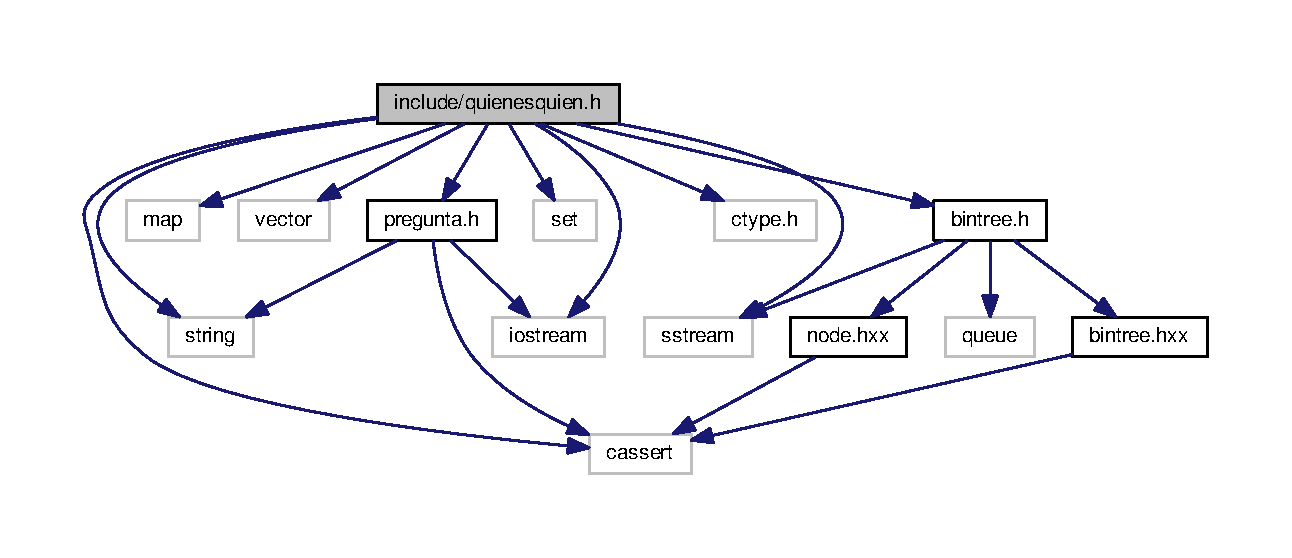
\includegraphics[width=350pt]{quienesquien_8h__incl}
\end{center}
\end{figure}
\subsection*{Clases}
\begin{DoxyCompactItemize}
\item 
class \hyperlink{classQuienEsQuien}{Quien\+Es\+Quien}
\begin{DoxyCompactList}\small\item\em T.\+D.\+A. \hyperlink{classQuienEsQuien}{Quien\+Es\+Quien}. \end{DoxyCompactList}\end{DoxyCompactItemize}
\subsection*{\textquotesingle{}defines\textquotesingle{}}
\begin{DoxyCompactItemize}
\item 
\#define {\bfseries D\+E\+B\+U\+G\+\_\+\+Q\+U\+I\+E\+N\+E\+S\+Q\+U\+I\+EN}~0\hypertarget{quienesquien_8h_ae6c0205a5b1ad44e00fe693e3c7f7dbd}{}\label{quienesquien_8h_ae6c0205a5b1ad44e00fe693e3c7f7dbd}

\end{DoxyCompactItemize}


\subsection{Descripción detallada}
Fichero cabecera del \hyperlink{classQuienEsQuien}{Quien\+Es\+Quien}. 

Almacena el �rbol de preguntas para jugar al �\+Qui�n es qui�n?.

\begin{DoxyAuthor}{Autor}
Elvira Castillo Fernández (Grupo D3) 

Alejandro Jerónimo Fuentes (Grupo B1) 
\end{DoxyAuthor}

%--- End generated contents ---

% Index
\backmatter
\newpage
\phantomsection
\clearemptydoublepage
\addcontentsline{toc}{chapter}{Índice}
\printindex

\end{document}
